\subsection{WDM signal}

In this study, we examined a fiber optic line with a single channel WDM signal using a 16-quadrature amplitude modulation (16-QAM) symbol sequence at a symbol rate of $34\ [\textrm{GBd}]$ in a single polarization. The signal, shaped by a digital root-raised cosine (RRC) filter with a 0.1 roll-off factor, covered $12 \times 80\ [\textrm{km}]$ spans of standard single-mode fiber (SSFM). Signal average power $P_{\mathrm{ave}}$ varied between -25 and 6 dBm. Simulations, run in a noise-free environment, utilized an \gls{ssfm} model operating at a wavelength of $\lambda = 1550\ [\textrm{nm}]$ characterized by an attenuation coefficient $\alpha = 0.0\ [\textrm{dB}/\textrm{km}]$, a dispersion coefficient $D = 16.8\ \textrm{ps}/[\textrm{nm} \cdot \textrm{km}]$, and a nonlinear coefficient $\gamma = 1.2\ [\textrm{W} \cdot \textrm{km}]^{-1}$. For window processing, the CDC-window mode was employed with parameters: processing interval $T_{proc}$ is 32 symbols and dispersion side intervals $T_d = 300$ symbols.


\begin{figure}[h]
    \center{
        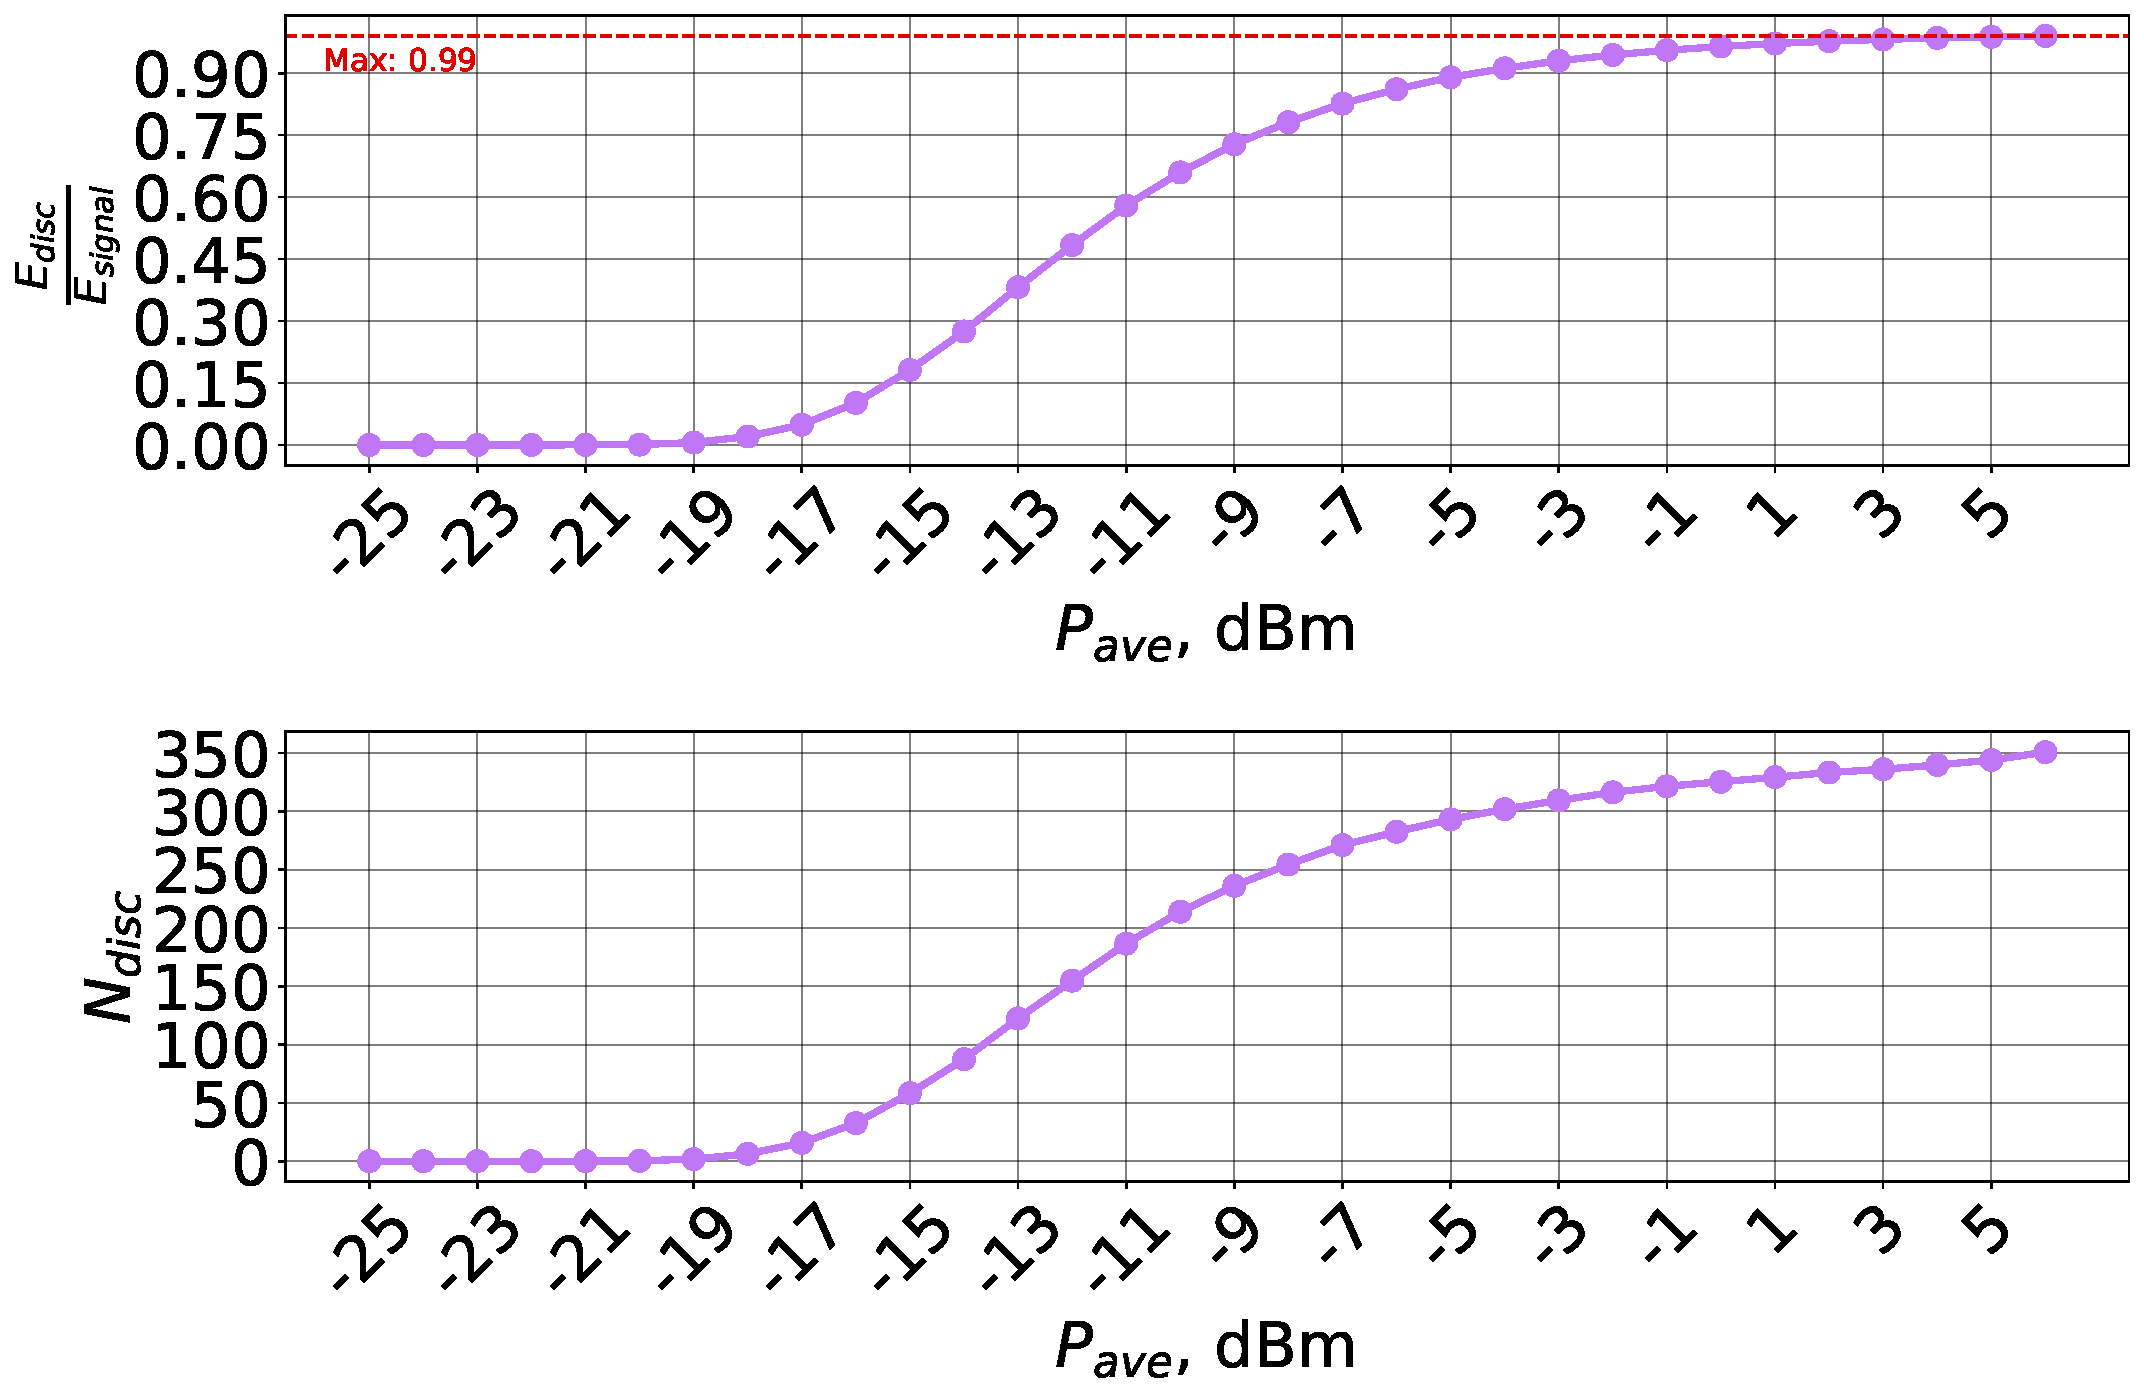
\includegraphics[width=0.9\linewidth]{images/soliton/wdm_trans/discrete_spectrum_vs_power.pdf}
    }
    \caption{\textbf{Upper}: Soliton energy proportion in WDM signal. \textbf{Lower}: Average soliton count at various power levels.}
    \label{fig:ds_vs_power}
\end{figure}

The upper image in Fig.~\ref{fig:ds_vs_power} illustrates the proportion of signal energy that comprises the soliton component within a WDM signal. The lower image displays the average quantity of solitons at specific power levels. These representations are based on the statistics of 1024 distinct windowed intervals for the WDM signal. It is important to note that the step shift is equivalent to \( T_{\text{proc}} \), resulting in overlapping windows. However, this overlap does not affect the overall trend, as the contributions from identical solitons, which may be counted multiple times, are averaged out. Consequently, we observe consistent behavior for non-overlapping intervals as well.

At lower average signal power levels, the soliton component is absent, with both the number and energy of solitons being zero, as expected. Interestingly, an increase in power leads to a rise in the energy allocated to the soliton component. Commencing at approximately -20 dBm, the count begins to ascend, followed by a corresponding increase in the soliton energy fraction. Near the 1-3 dBm range, almost 99\% of the energy attributed to solitons within the signal, and this proportion remains stable even as the average power level continues to increase (up to the maximum observed level of 6 dBm).

The number of solitons does not saturate at the same level (around 1 dBm) and continues to grow with an increase in average power. Notably, even at 5 dBm and 6 dBm, a distinction in the soliton count is evident. This phenomenon suggests that, beyond a certain saturation point of power, where the majority of the energy is soliton-associated, the number of solitons can still proliferate. This implies that the emergence of higher-energy solitons becomes unlikely, while the system favors an increase in lower-energy solitons that collectively assimilate the available energy.

From a physical perspective, systems gravitate towards a state of minimal energy, which is more readily achieved by integrating multiple low-energy solitons rather than a combination of a few high-energy and several very low-energy solitons. Statistically, it is also more likely to obtain uniform results across different signal realizations with typical energy levels than with extreme soliton power values. These observations foster a discussion regarding the implications of the data, setting the stage for following validation of our preliminary interpretations.


\begin{figure}[tpb]
    \begin{minipage}[h]{0.33\linewidth}
    \center{
        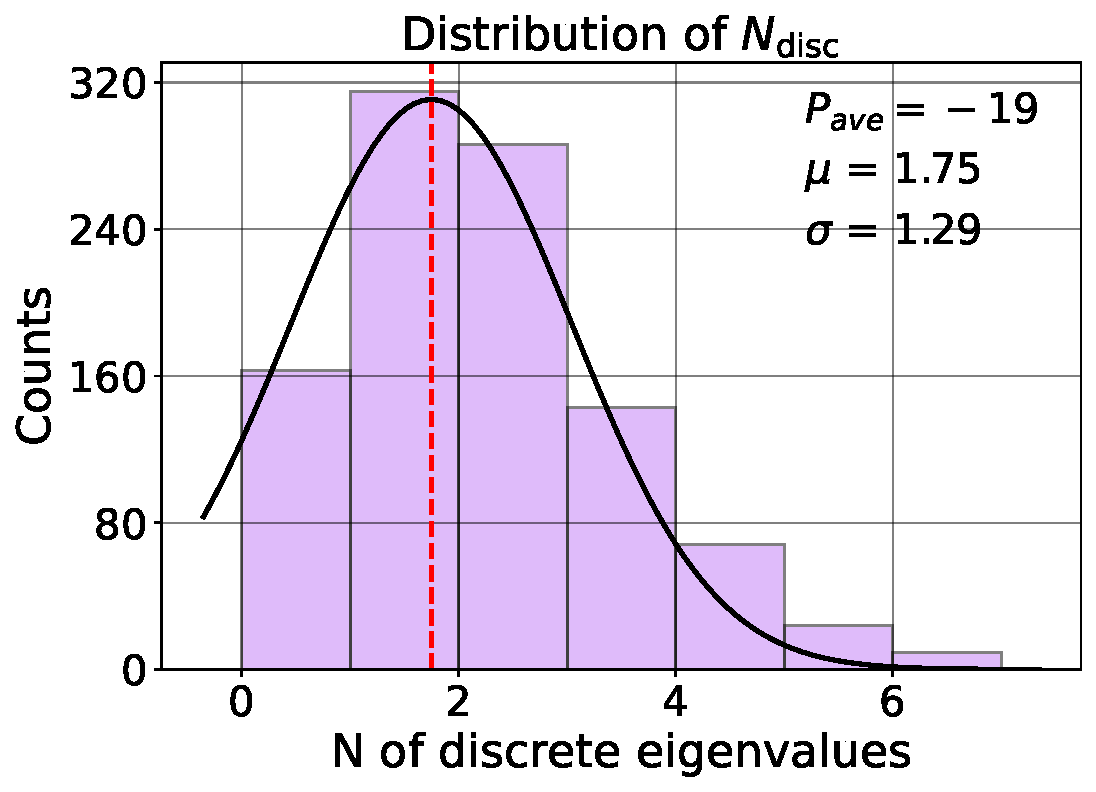
\includegraphics[width=1\linewidth]{images/soliton/wdm_trans/discrete_spectrum_solo_pavedbm_-19.pdf} \\
    }
    \end{minipage}
    \begin{minipage}[h]{0.33\linewidth}
    \center{
        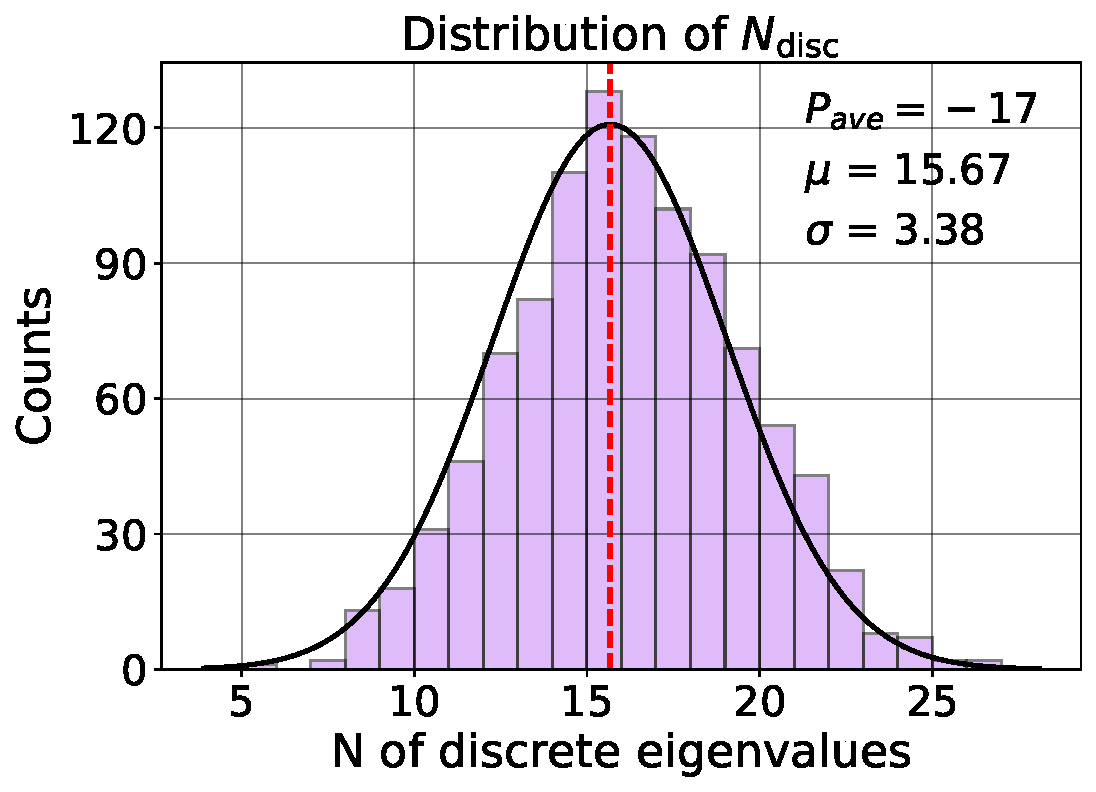
\includegraphics[width=1\linewidth]{images/soliton/wdm_trans/discrete_spectrum_solo_pavedbm_-17.pdf} \\
    }
    \end{minipage}
    \begin{minipage}[h]{0.33\linewidth}
    \center{
        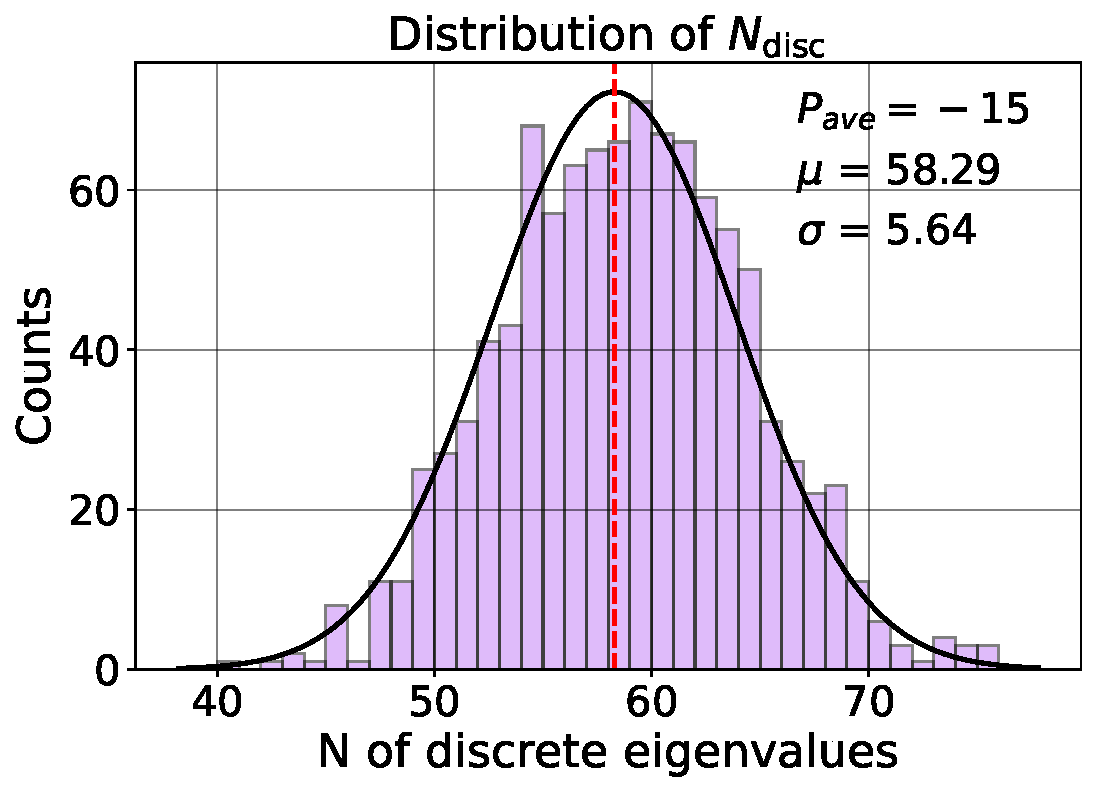
\includegraphics[width=1\linewidth]{images/soliton/wdm_trans/discrete_spectrum_solo_pavedbm_-15.pdf} \\
    }
    \end{minipage}

    \begin{minipage}[h]{0.33\linewidth}
    \center{
        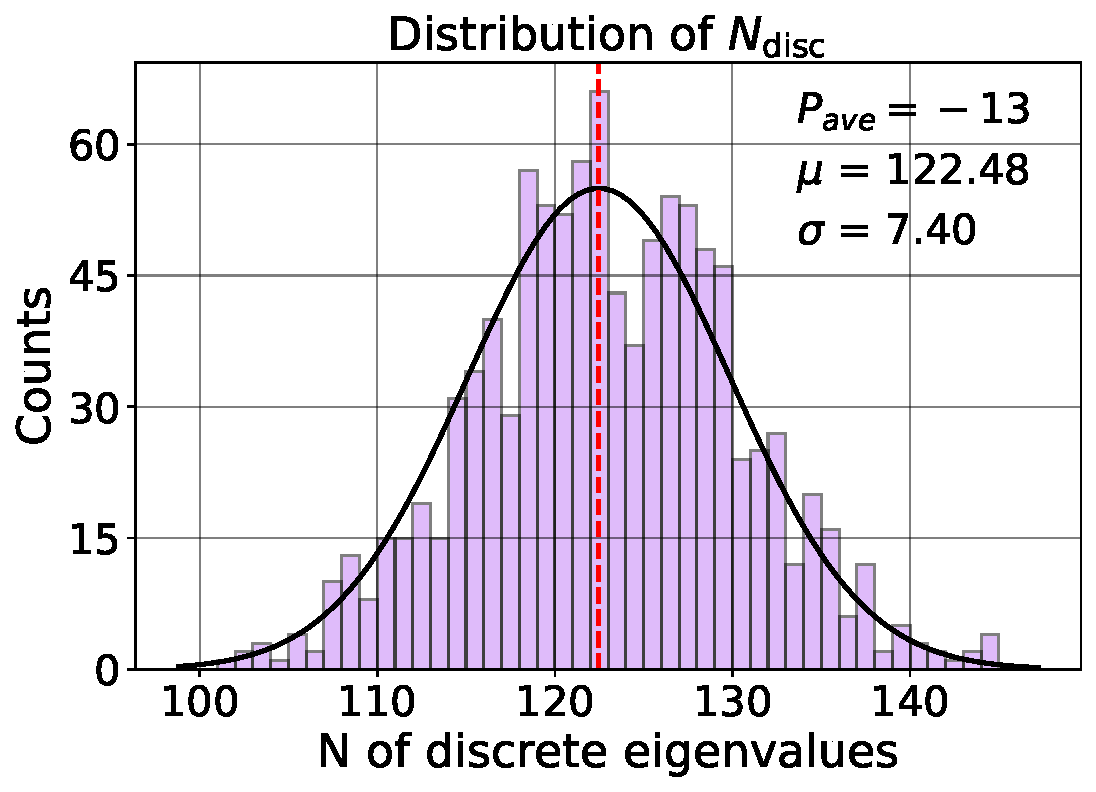
\includegraphics[width=1\linewidth]{images/soliton/wdm_trans/discrete_spectrum_solo_pavedbm_-13.pdf} \\
    }
    \end{minipage}
    \begin{minipage}[h]{0.33\linewidth}
    \center{
        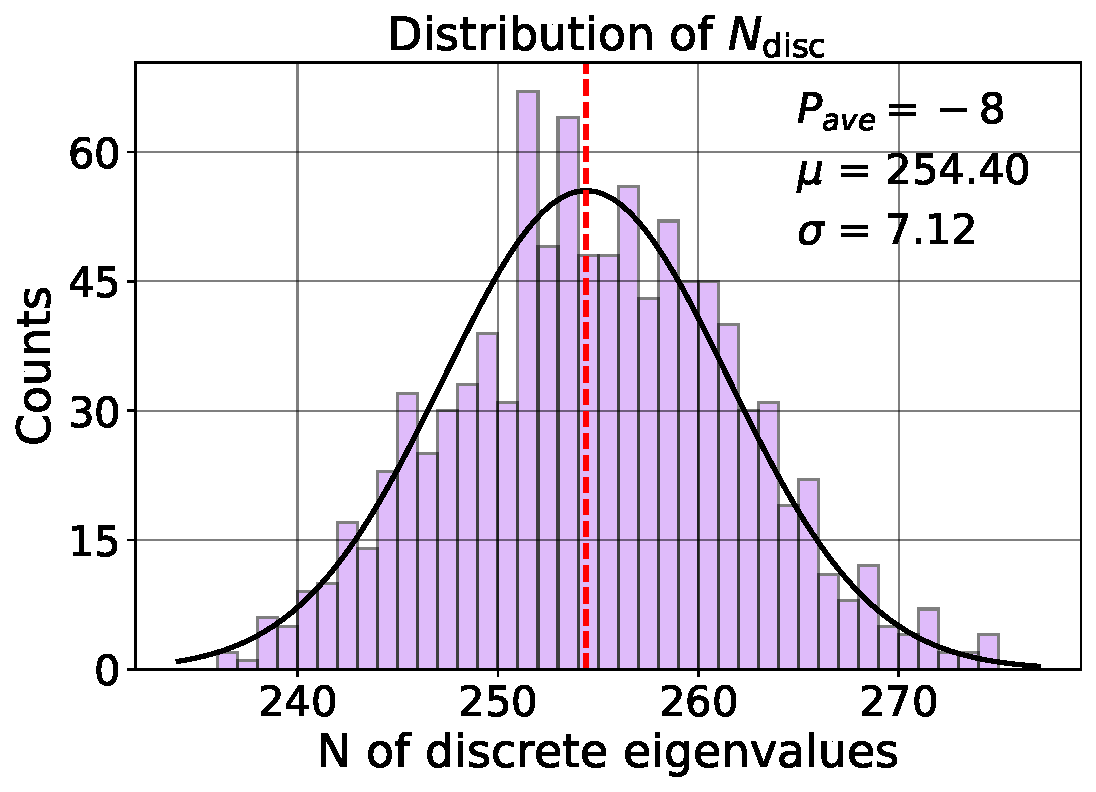
\includegraphics[width=1\linewidth]{images/soliton/wdm_trans/discrete_spectrum_solo_pavedbm_-8.pdf} \\
    }
    \end{minipage}
    \begin{minipage}[h]{0.33\linewidth}
    \center{
        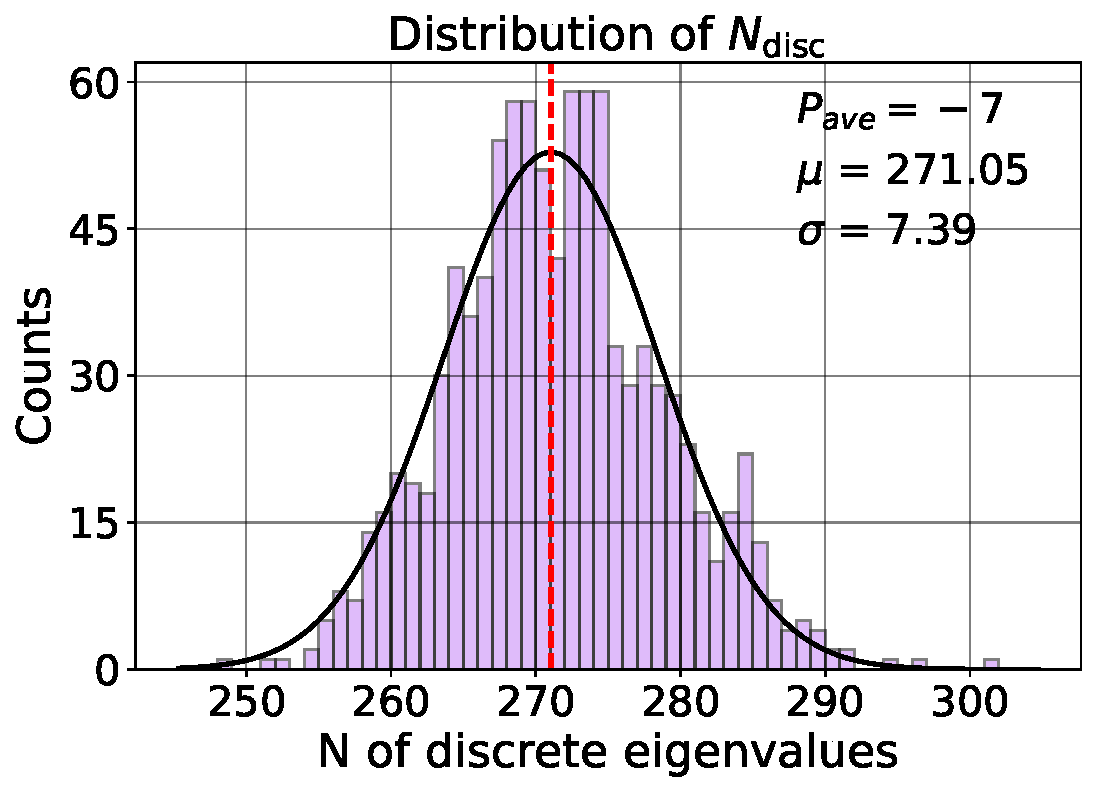
\includegraphics[width=1\linewidth]{images/soliton/wdm_trans/discrete_spectrum_solo_pavedbm_-7.pdf} \\
    }
    \end{minipage}

    \begin{minipage}[h]{0.33\linewidth}
    \center{
        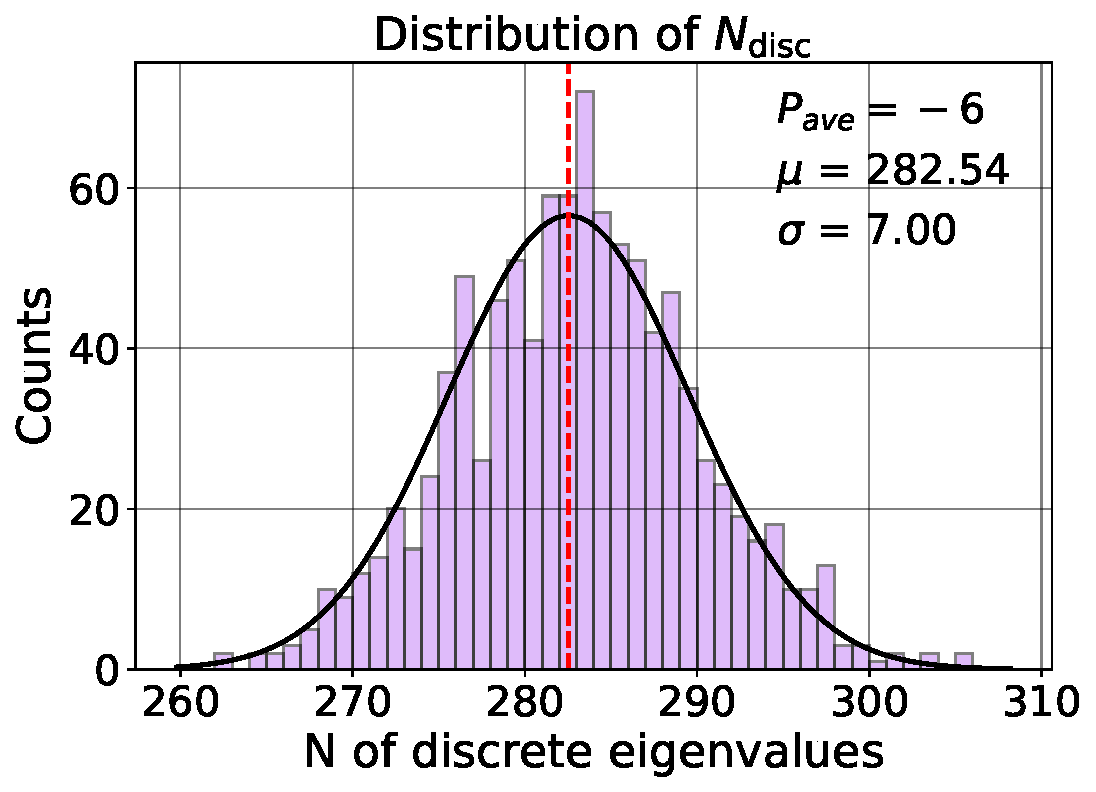
\includegraphics[width=1\linewidth]{images/soliton/wdm_trans/discrete_spectrum_solo_pavedbm_-6.pdf} \\
    }
    \end{minipage}
    \begin{minipage}[h]{0.33\linewidth}
    \center{
        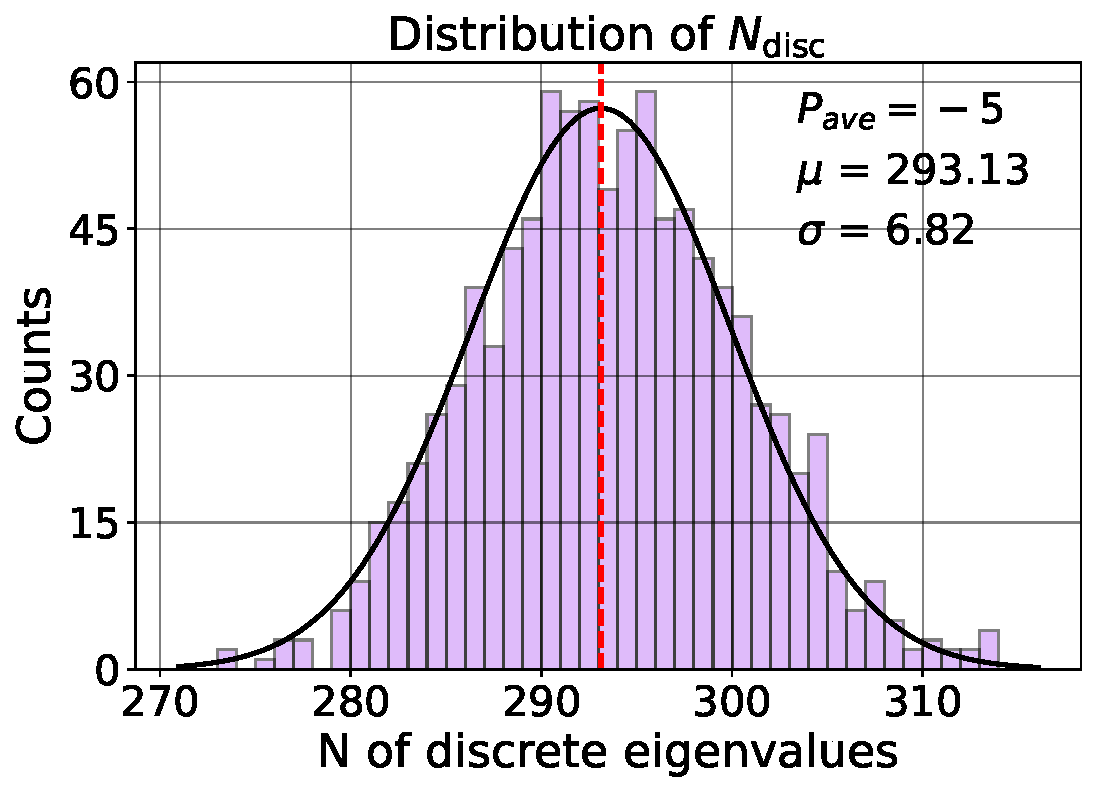
\includegraphics[width=1\linewidth]{images/soliton/wdm_trans/discrete_spectrum_solo_pavedbm_-5.pdf} \\
    }
    \end{minipage}
    \begin{minipage}[h]{0.33\linewidth}
    \center{
        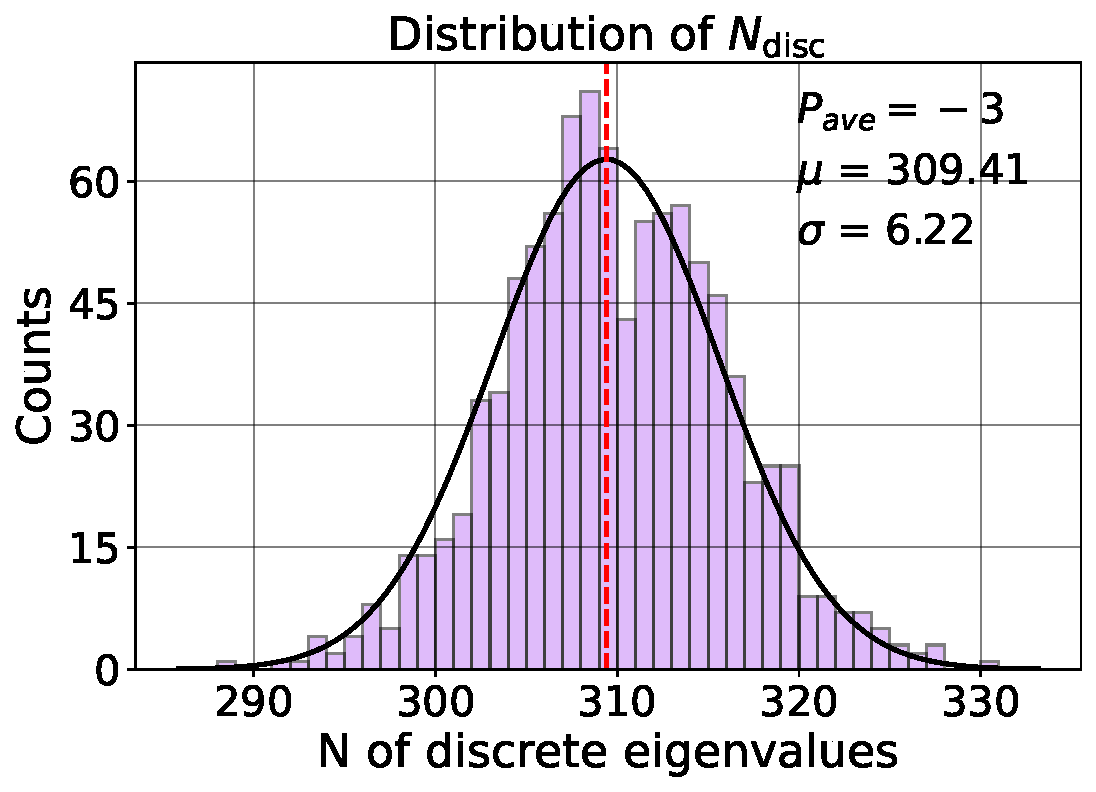
\includegraphics[width=1\linewidth]{images/soliton/wdm_trans/discrete_spectrum_solo_pavedbm_-3.pdf} \\
    }
    \end{minipage}

    \begin{minipage}[h]{0.33\linewidth}
    \center{
        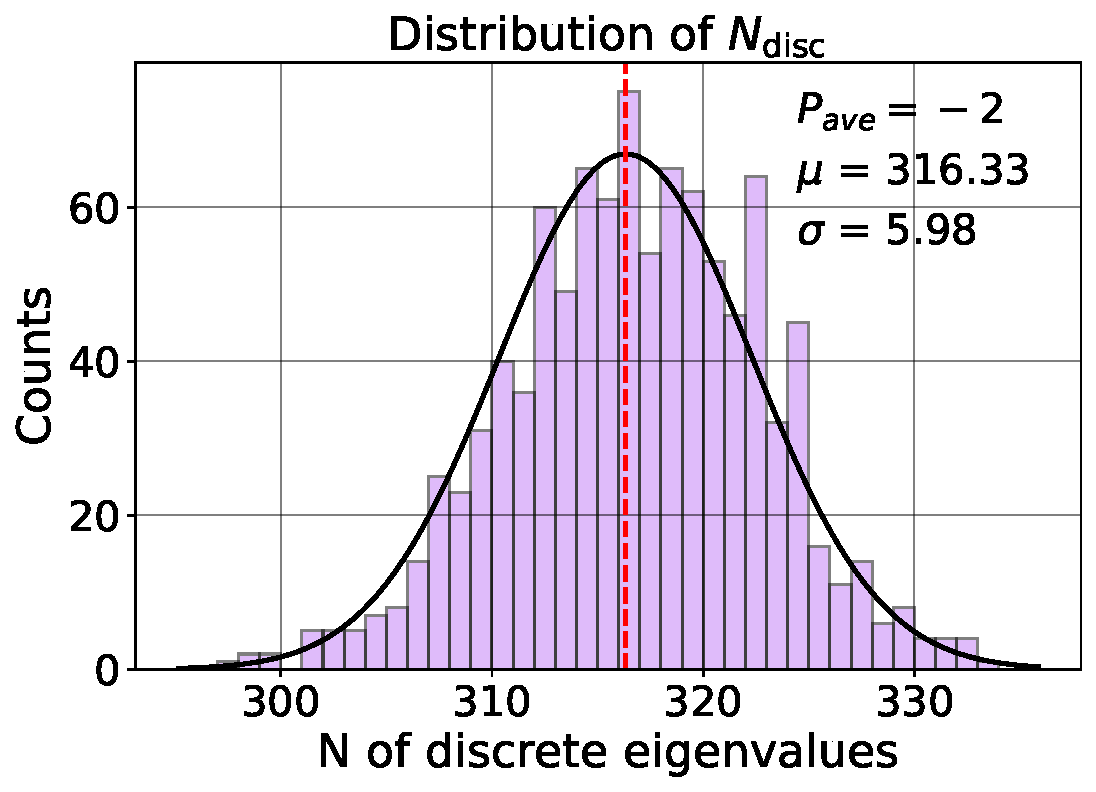
\includegraphics[width=1\linewidth]{images/soliton/wdm_trans/discrete_spectrum_solo_pavedbm_-2.pdf} \\
    }
    \end{minipage}
    \begin{minipage}[h]{0.33\linewidth}
    \center{
        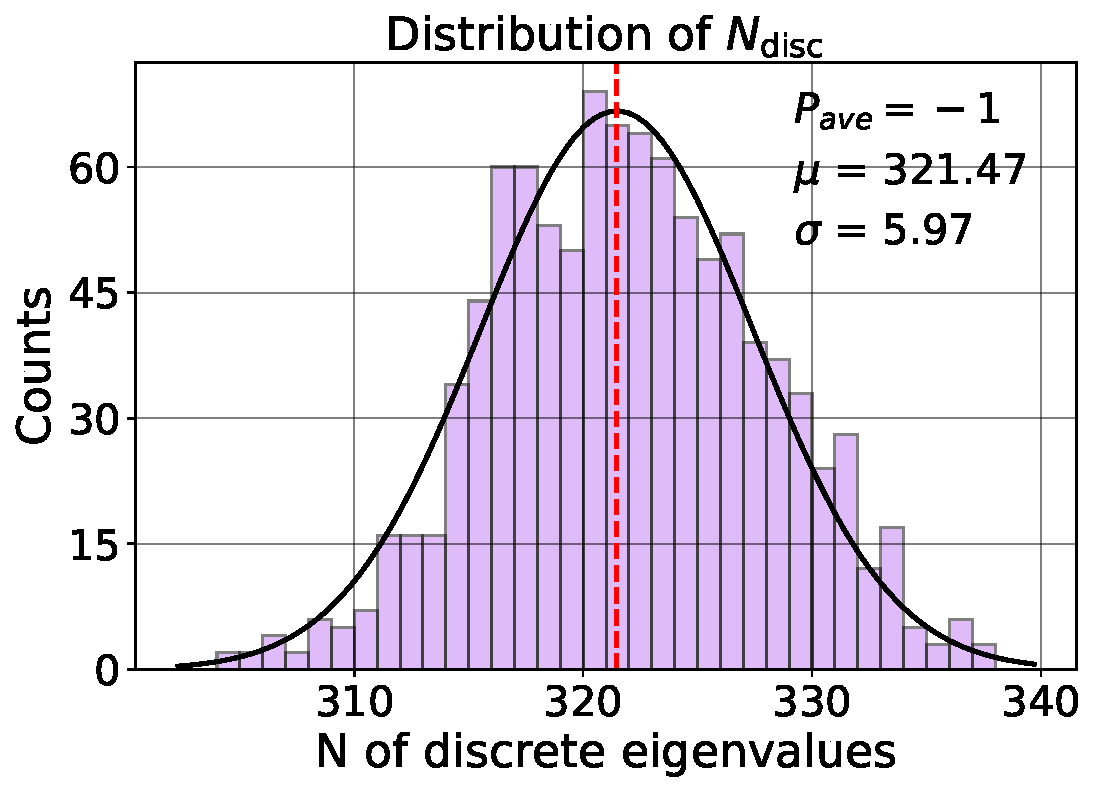
\includegraphics[width=1\linewidth]{images/soliton/wdm_trans/discrete_spectrum_solo_pavedbm_-1.pdf} \\
    }
    \end{minipage}
    \begin{minipage}[h]{0.33\linewidth}
    \center{
        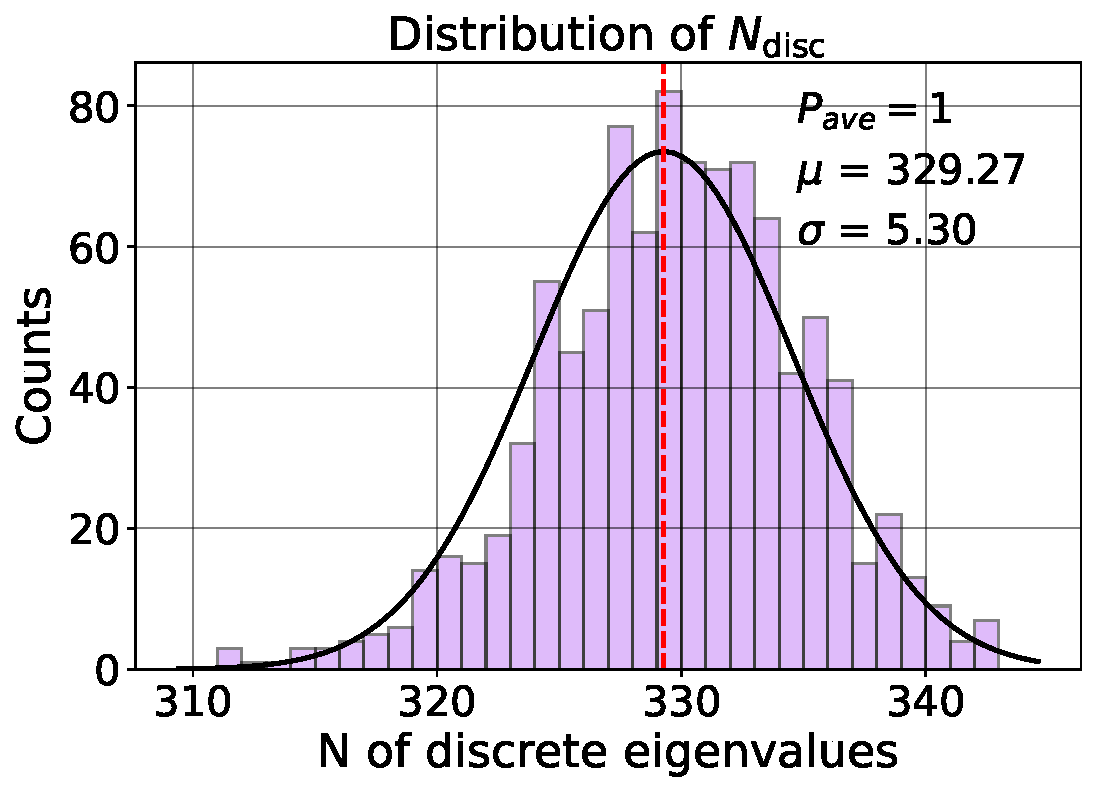
\includegraphics[width=1\linewidth]{images/soliton/wdm_trans/discrete_spectrum_solo_pavedbm_1.pdf} \\
    }
    \end{minipage}

    \begin{minipage}[h]{0.33\linewidth}
    \center{
        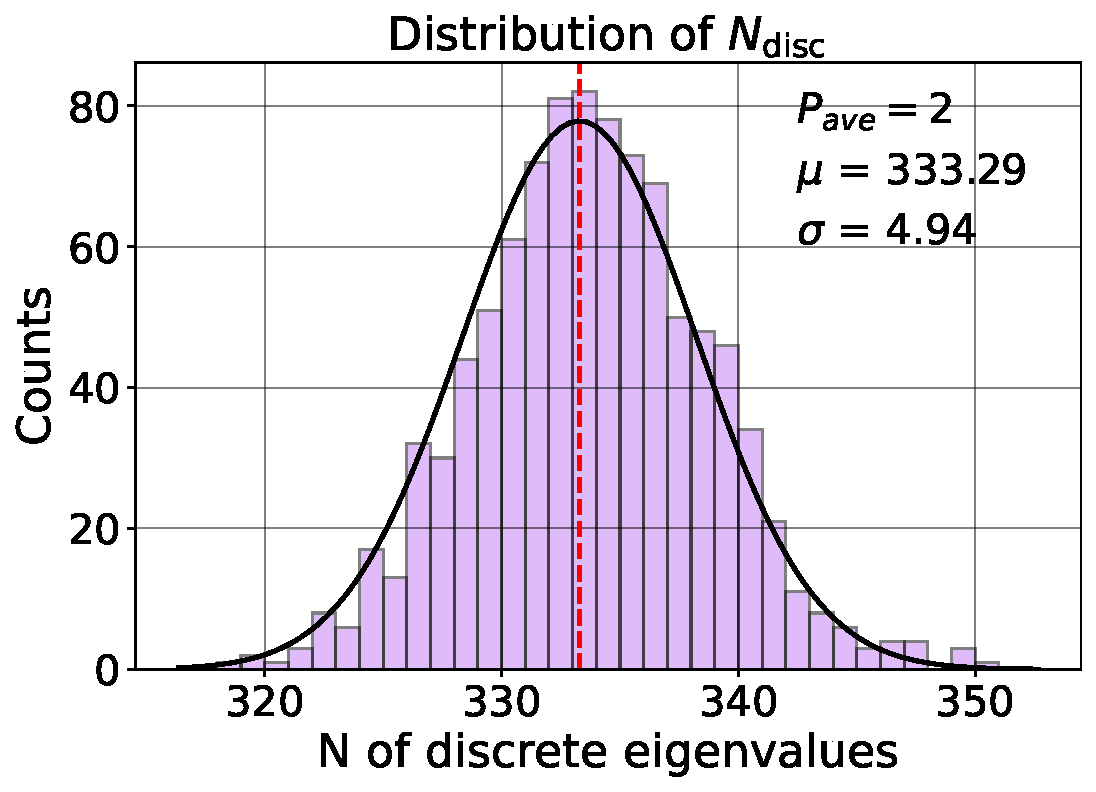
\includegraphics[width=1\linewidth]{images/soliton/wdm_trans/discrete_spectrum_solo_pavedbm_2.pdf} \\
    }
    \end{minipage}
    \begin{minipage}[h]{0.33\linewidth}
    \center{
        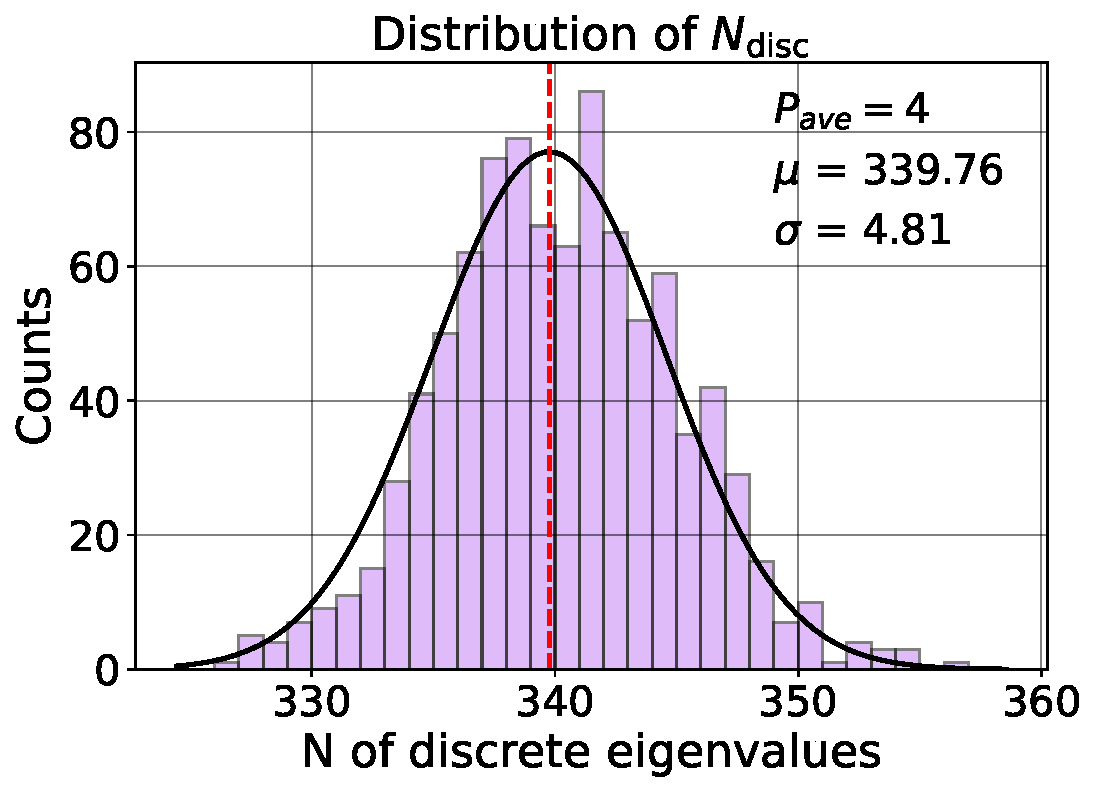
\includegraphics[width=1\linewidth]{images/soliton/wdm_trans/discrete_spectrum_solo_pavedbm_4.pdf} \\
    }
    \end{minipage}
    \begin{minipage}[h]{0.33\linewidth}
    \center{
        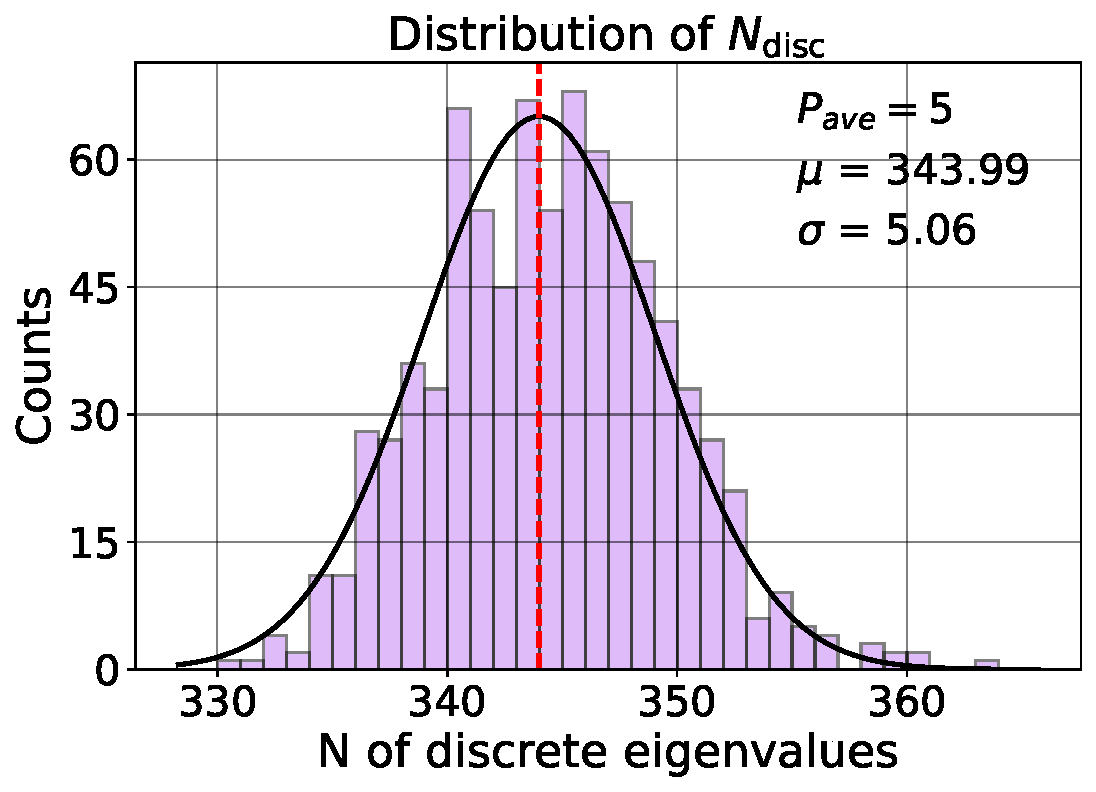
\includegraphics[width=1\linewidth]{images/soliton/wdm_trans/discrete_spectrum_solo_pavedbm_5.pdf} \\
    }
    \end{minipage}
    \caption{Comparison of soliton distibution for WDM signal with differnt average signal power.}
    \label{fig:wdm_trans_sol}
\end{figure}

Figure~\ref{fig:wdm_trans_sol} displays the distribution of discrete points in the NF spectrum, which corresponds to the number of solitons, across different average signal power levels. Starting with the upper left plot at the lowest power of \(-19\) dBm, the power increases from one plot to the next, culminating in the lower left figure at the highest power of \(5\) dBm. This range of power levels, as seen in Fig.~\ref{fig:ds_vs_power}, spans from scenarios with nearly no solitons to those where the power is predominantly in soliton form.

% TODO: change equation number
Additionally, Fig.~\ref{fig:wdm_trans_sol_with_max_eigen} complements the previous figure by presenting the distribution of the maximum imaginary part of the NF spectrum, which is directly related to soliton power (refer to Eq. 5). Our prior analysis on soliton content within single symbols indicates that certain power levels, particularly at the boundaries like \(-20\) dBm (Fig.~\ref{fig:wdm_trans_sol_with_max_eigen}) and \(-19\) dBm (first panel of Fig.~\ref{fig:wdm_trans_sol}), are not well-characterized by a Gaussian distribution. In these instances, a Poisson distribution offers a more accurate representation.

Excluding the borderline power levels up to \(-16\) to \(-15\) dBm, where a Poisson distribution may still be more appropriate, we observe that the standard deviation of the Gaussian distribution tends to decrease with increasing power. For power levels above this range, our preliminary data suggests a Gaussian standard deviation in the vicinity of \(7.0\) to \(7.4\). This value narrows to around \(6.0\) for power levels near \(-2\) to \(-1\) dBm, and even further to \(5.0\) for power levels between \(2\) and \(5\) dBm.

This trend hints at a region of stability where the occurrence of solitons is statistically more predictable and exhibits less variation. This stability may indicate the formation of physical structures akin to a ``soliton gas'', where solitons exhibit particle-like behavior, and thermodynamic principles could potentially apply.

At \(6\) dBm, as shown in the lower pane of Fig.~\ref{fig:wdm_trans_sol_with_max_eigen}, the standard deviation increases to \(5.75\). This could suggest either a statistical anomaly or the onset of a more complex system structure, necessitating further investigation. The concept of a soliton gas is an intriguing one that aligns with this observation, but it requires additional research to fully understand the relationship between soliton statistics and thermodynamic properties.

\begin{figure}[tpb]
    \begin{minipage}[h]{0.45\linewidth}
    \center{
        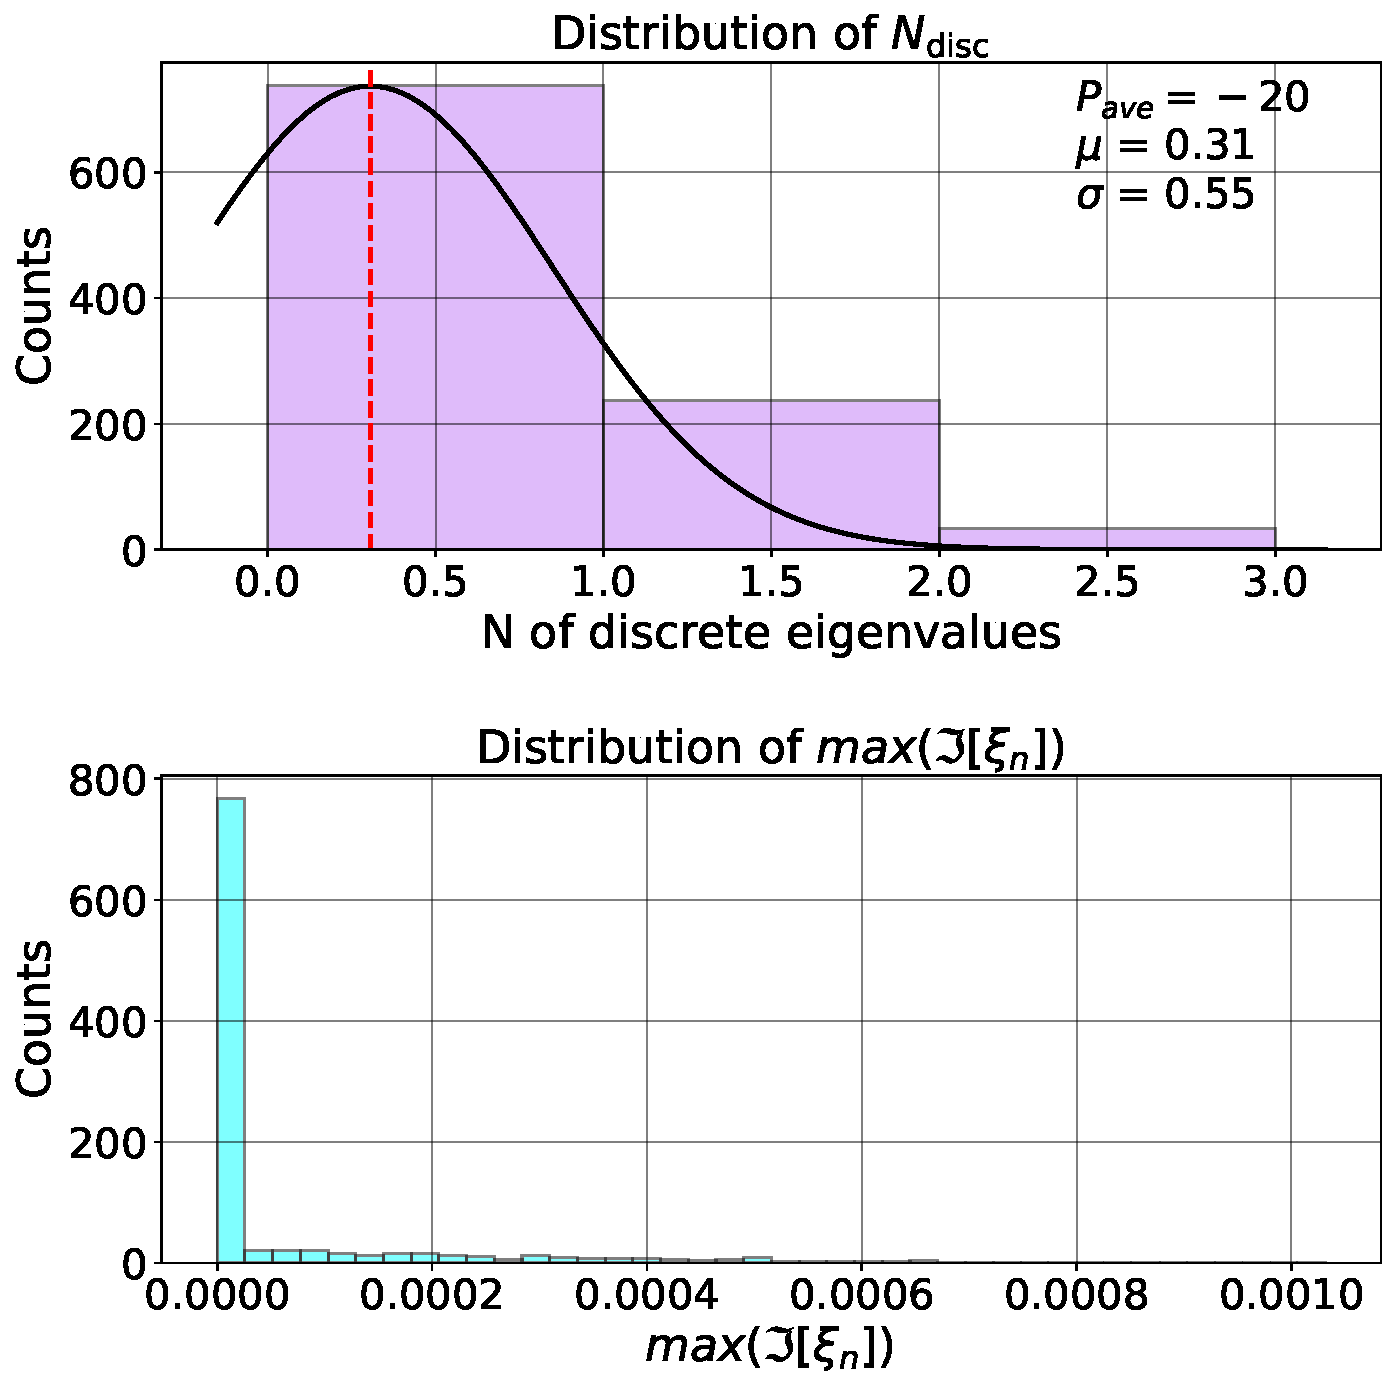
\includegraphics[width=1\linewidth]{images/soliton/wdm_trans/discrete_spectrum_pavedbm_-20.pdf} \\
    }
    \end{minipage}
    \hfill
    \begin{minipage}[h]{0.45\linewidth}
    \center{
        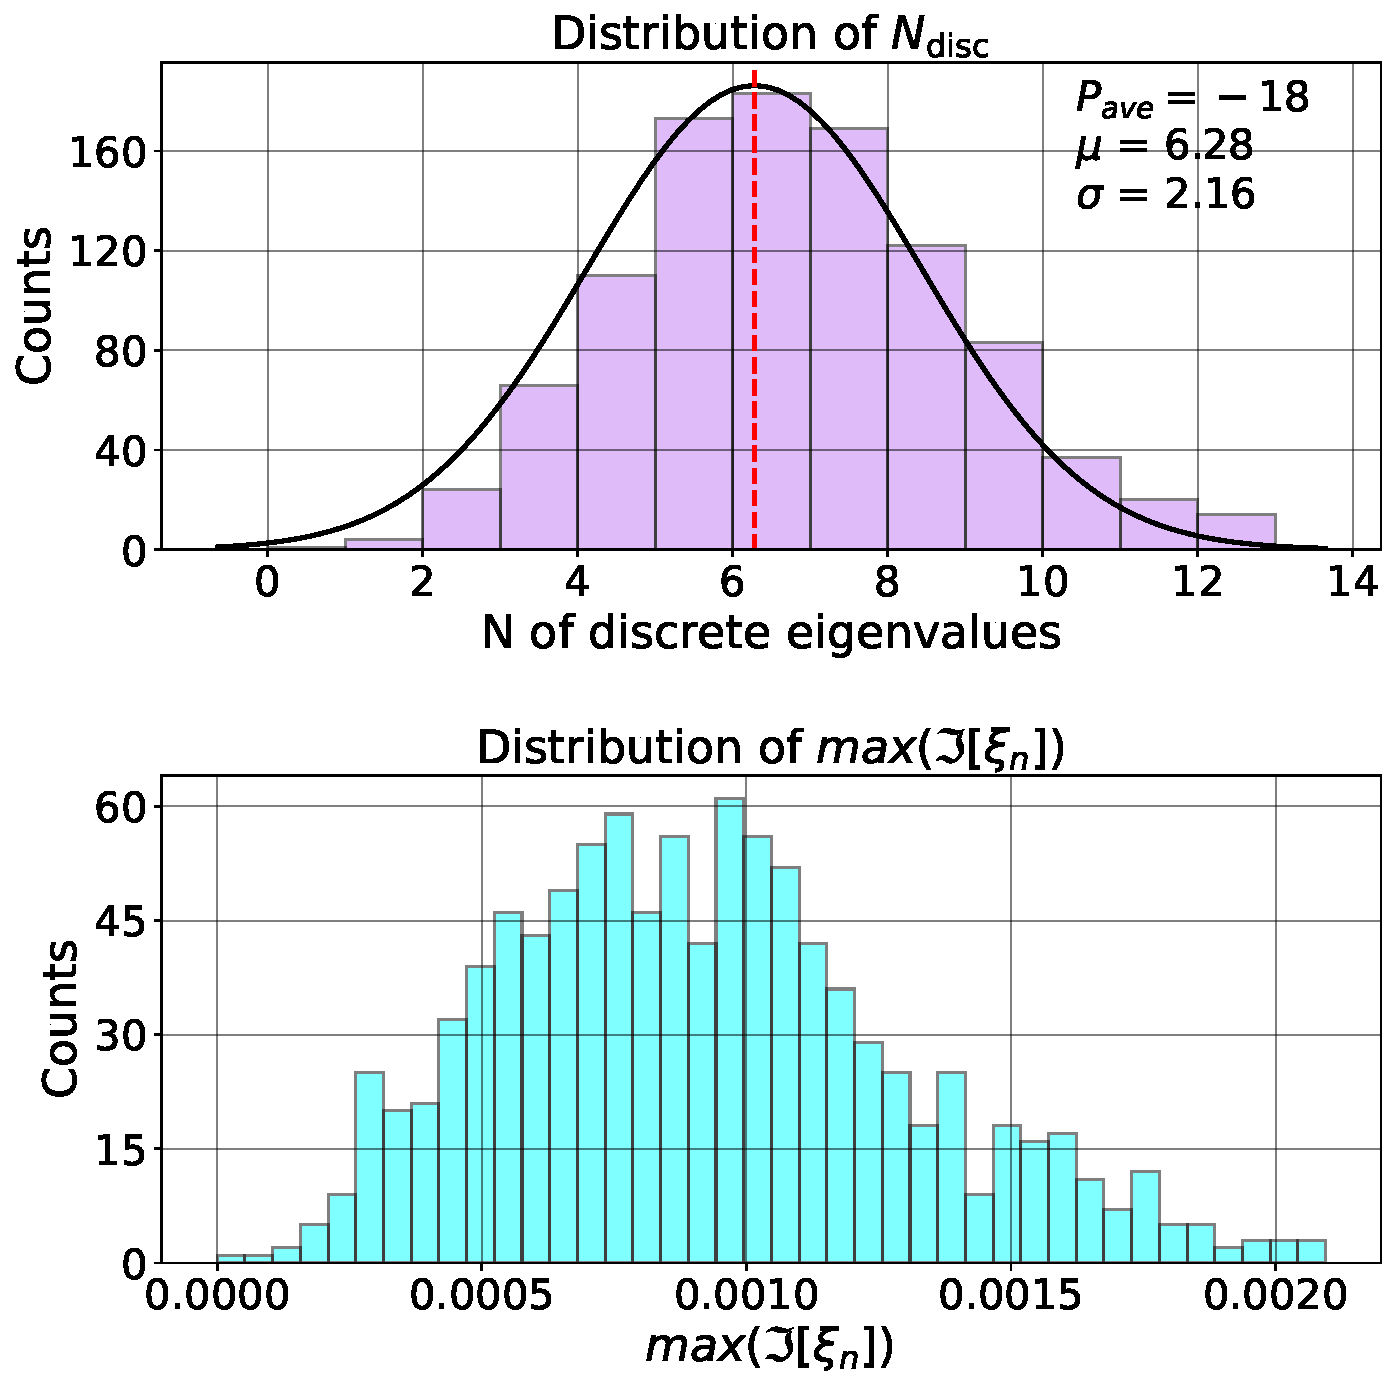
\includegraphics[width=1\linewidth]{images/soliton/wdm_trans/discrete_spectrum_pavedbm_-18.pdf} \\
    }
    \end{minipage}

    \begin{minipage}[h]{0.45\linewidth}
    \center{
        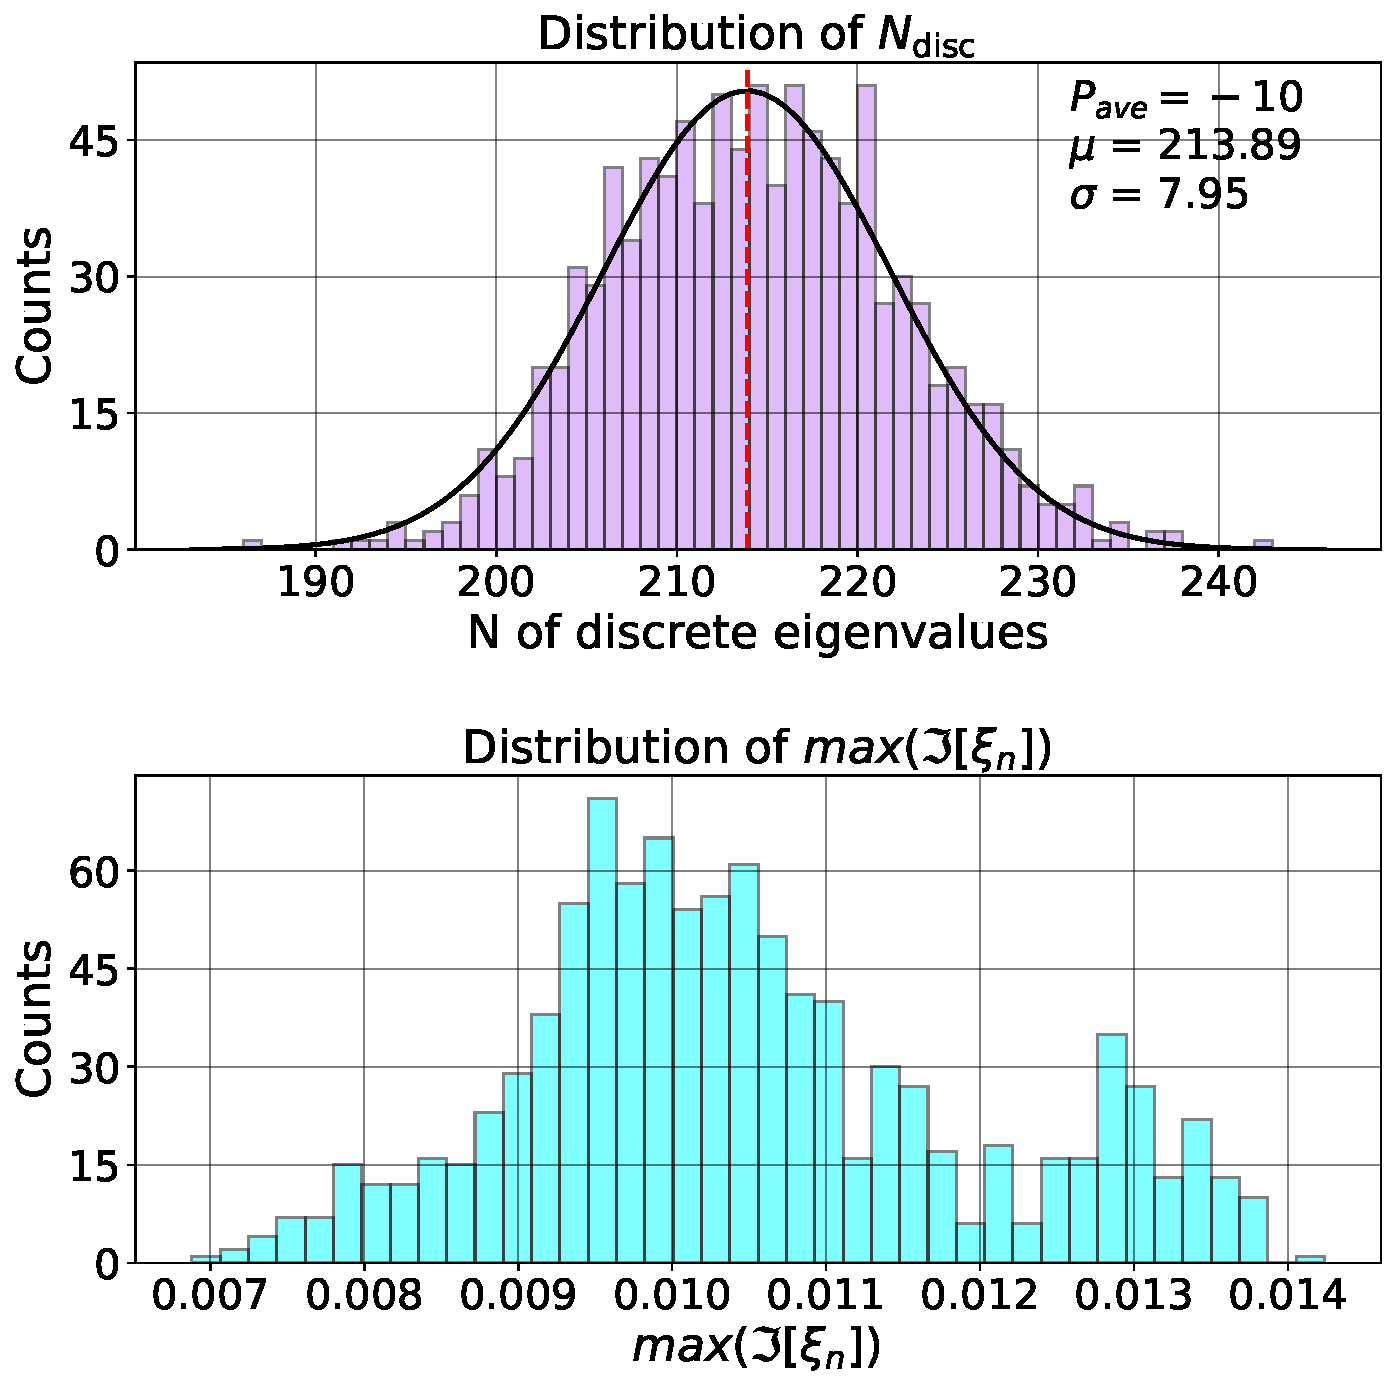
\includegraphics[width=1\linewidth]{images/soliton/wdm_trans/discrete_spectrum_pavedbm_-10.pdf} \\
    }
    \end{minipage}
    \hfill
    \begin{minipage}[h]{0.45\linewidth}
    \center{
        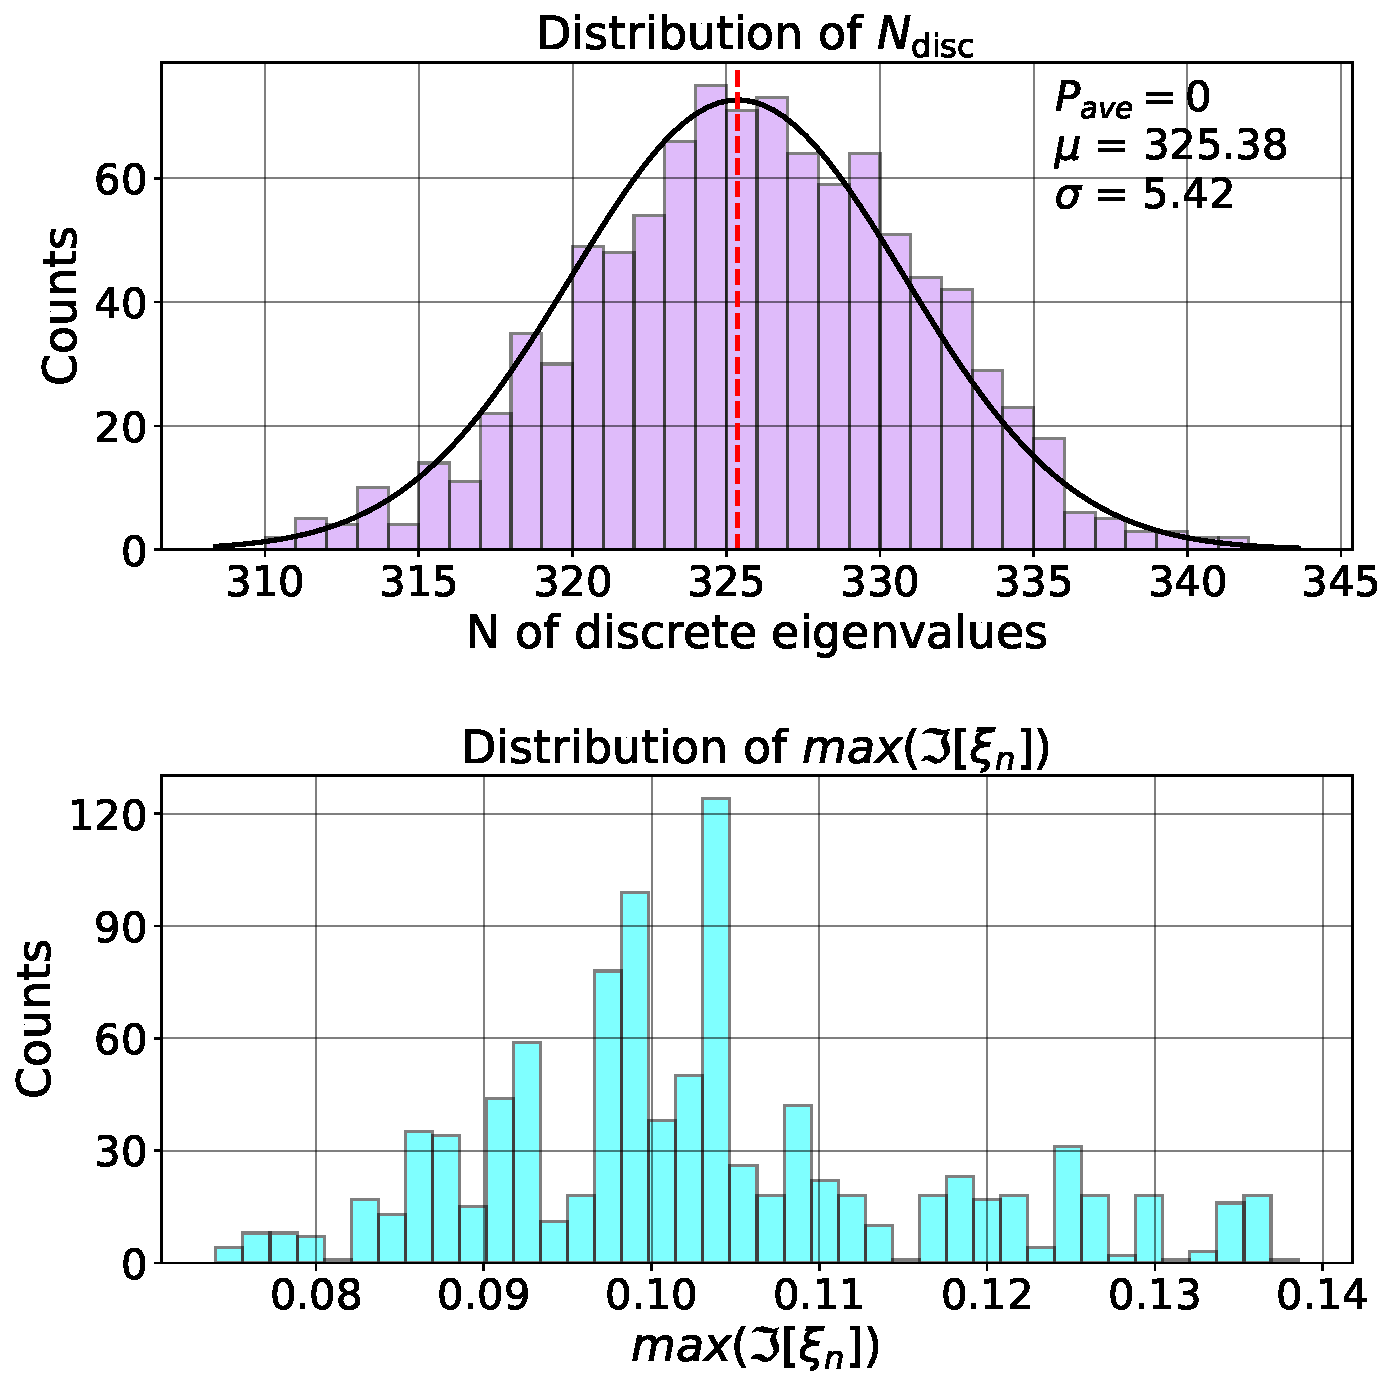
\includegraphics[width=1\linewidth]{images/soliton/wdm_trans/discrete_spectrum_pavedbm_0.pdf} \\
    }
    \end{minipage}

    \begin{minipage}[h]{0.45\linewidth}
    \center{
        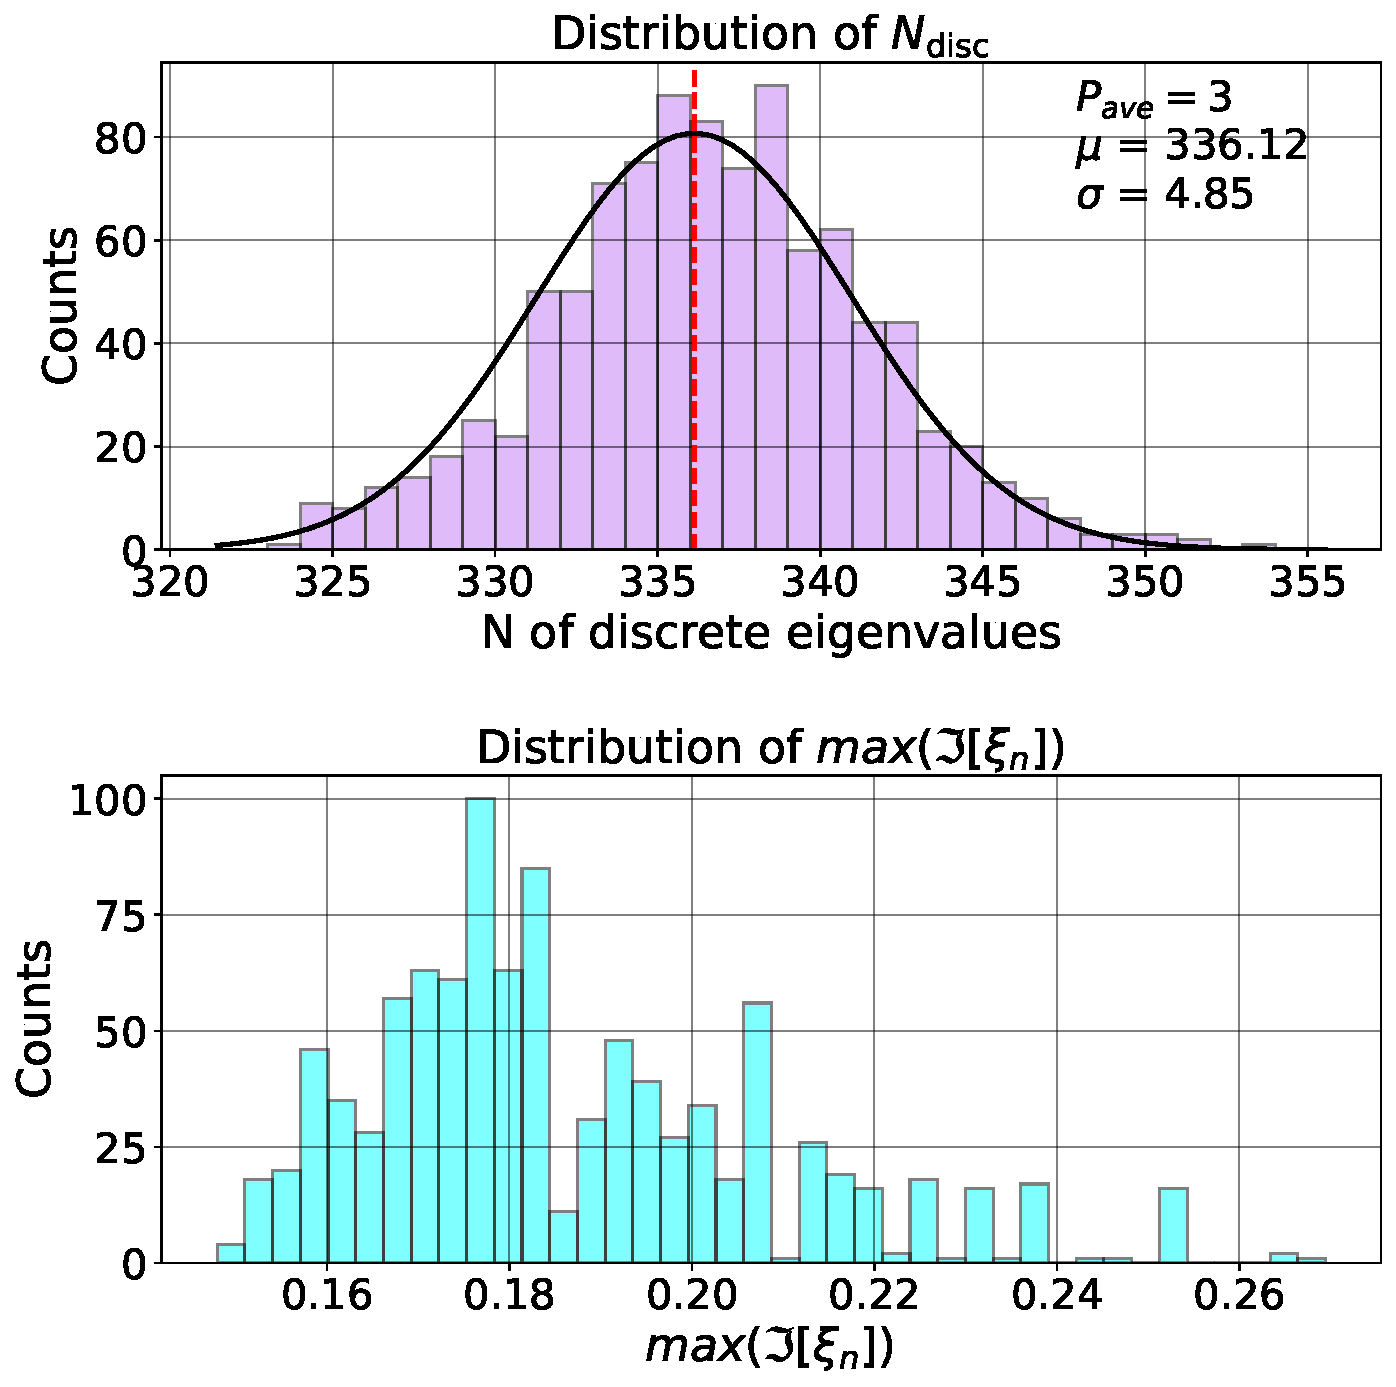
\includegraphics[width=1\linewidth]{images/soliton/wdm_trans/discrete_spectrum_pavedbm_3.pdf} \\
    }
    \end{minipage}
    \hfill
    \begin{minipage}[h]{0.45\linewidth}
    \center{
        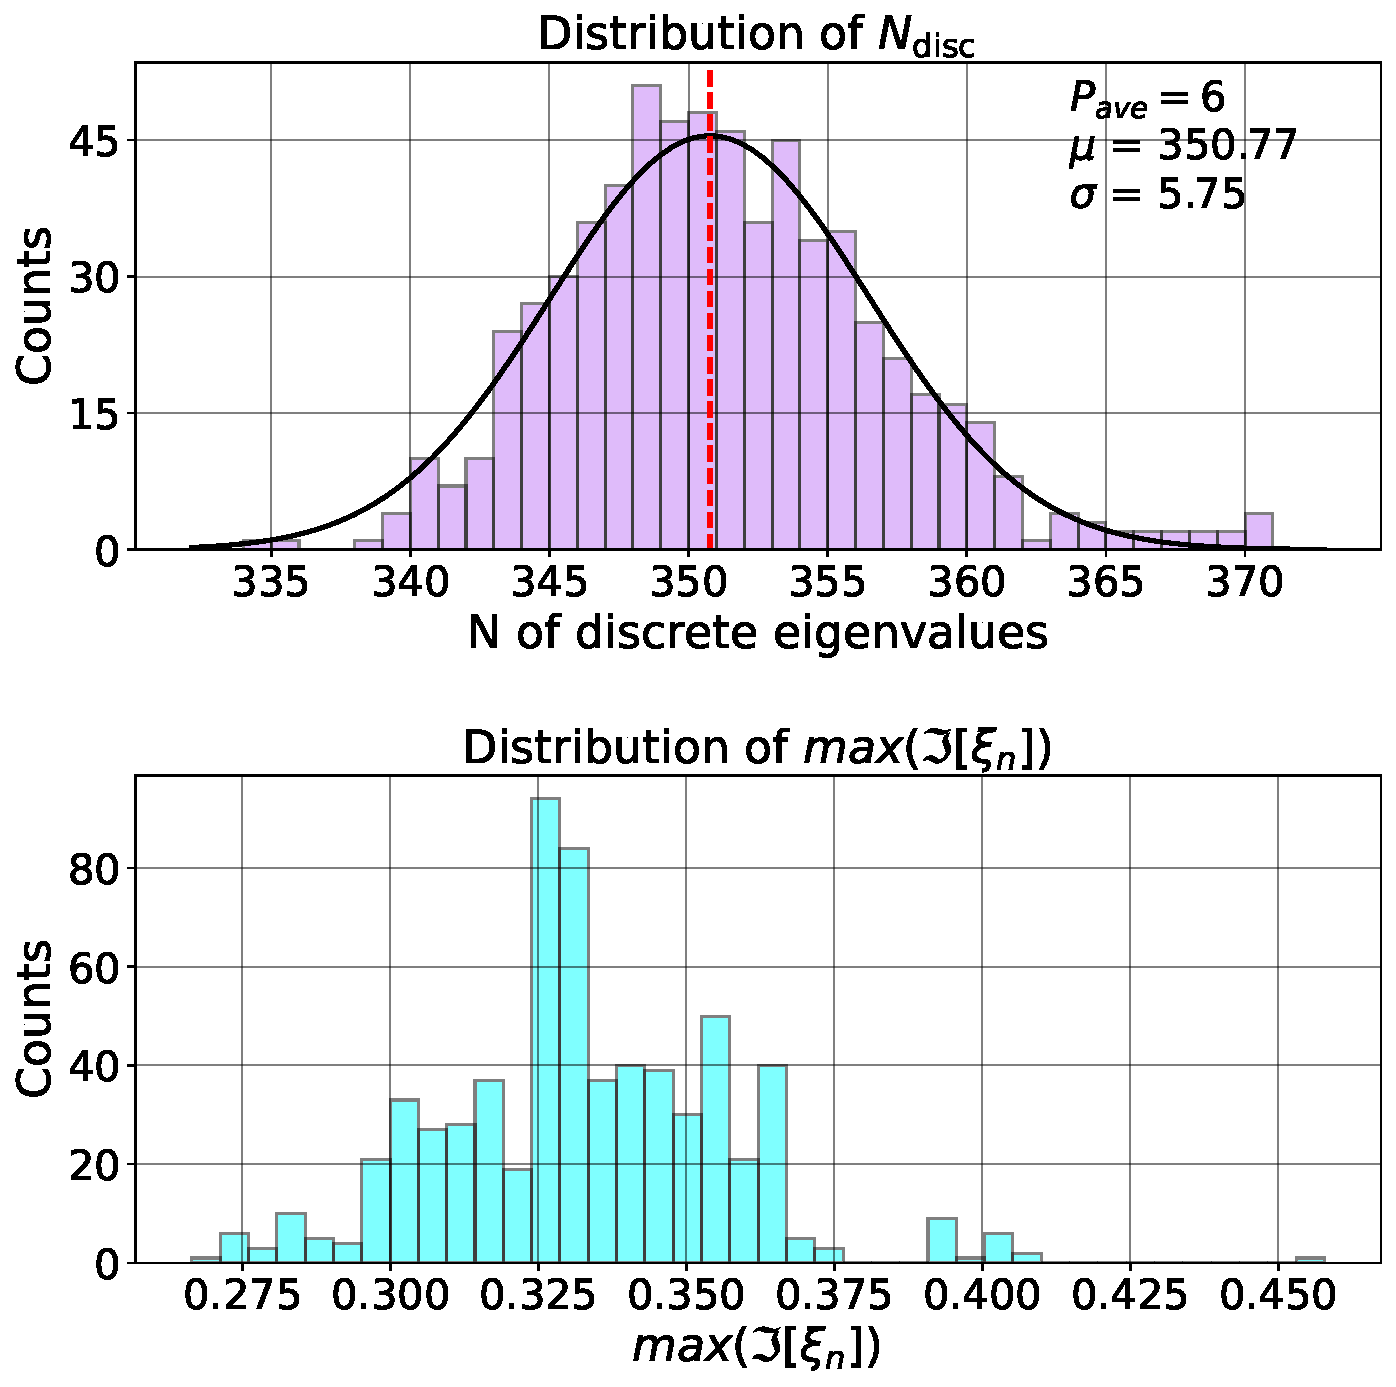
\includegraphics[width=1\linewidth]{images/soliton/wdm_trans/discrete_spectrum_pavedbm_6.pdf} \\
    }
    \end{minipage}
    \caption{Comparison of soliton distibution and distribution of maximum discrete eigenvalue}
    \label{fig:wdm_trans_sol_with_max_eigen}
\end{figure}

\begin{figure}[tpb]
    \begin{minipage}[h]{0.49\linewidth}
    \center{
        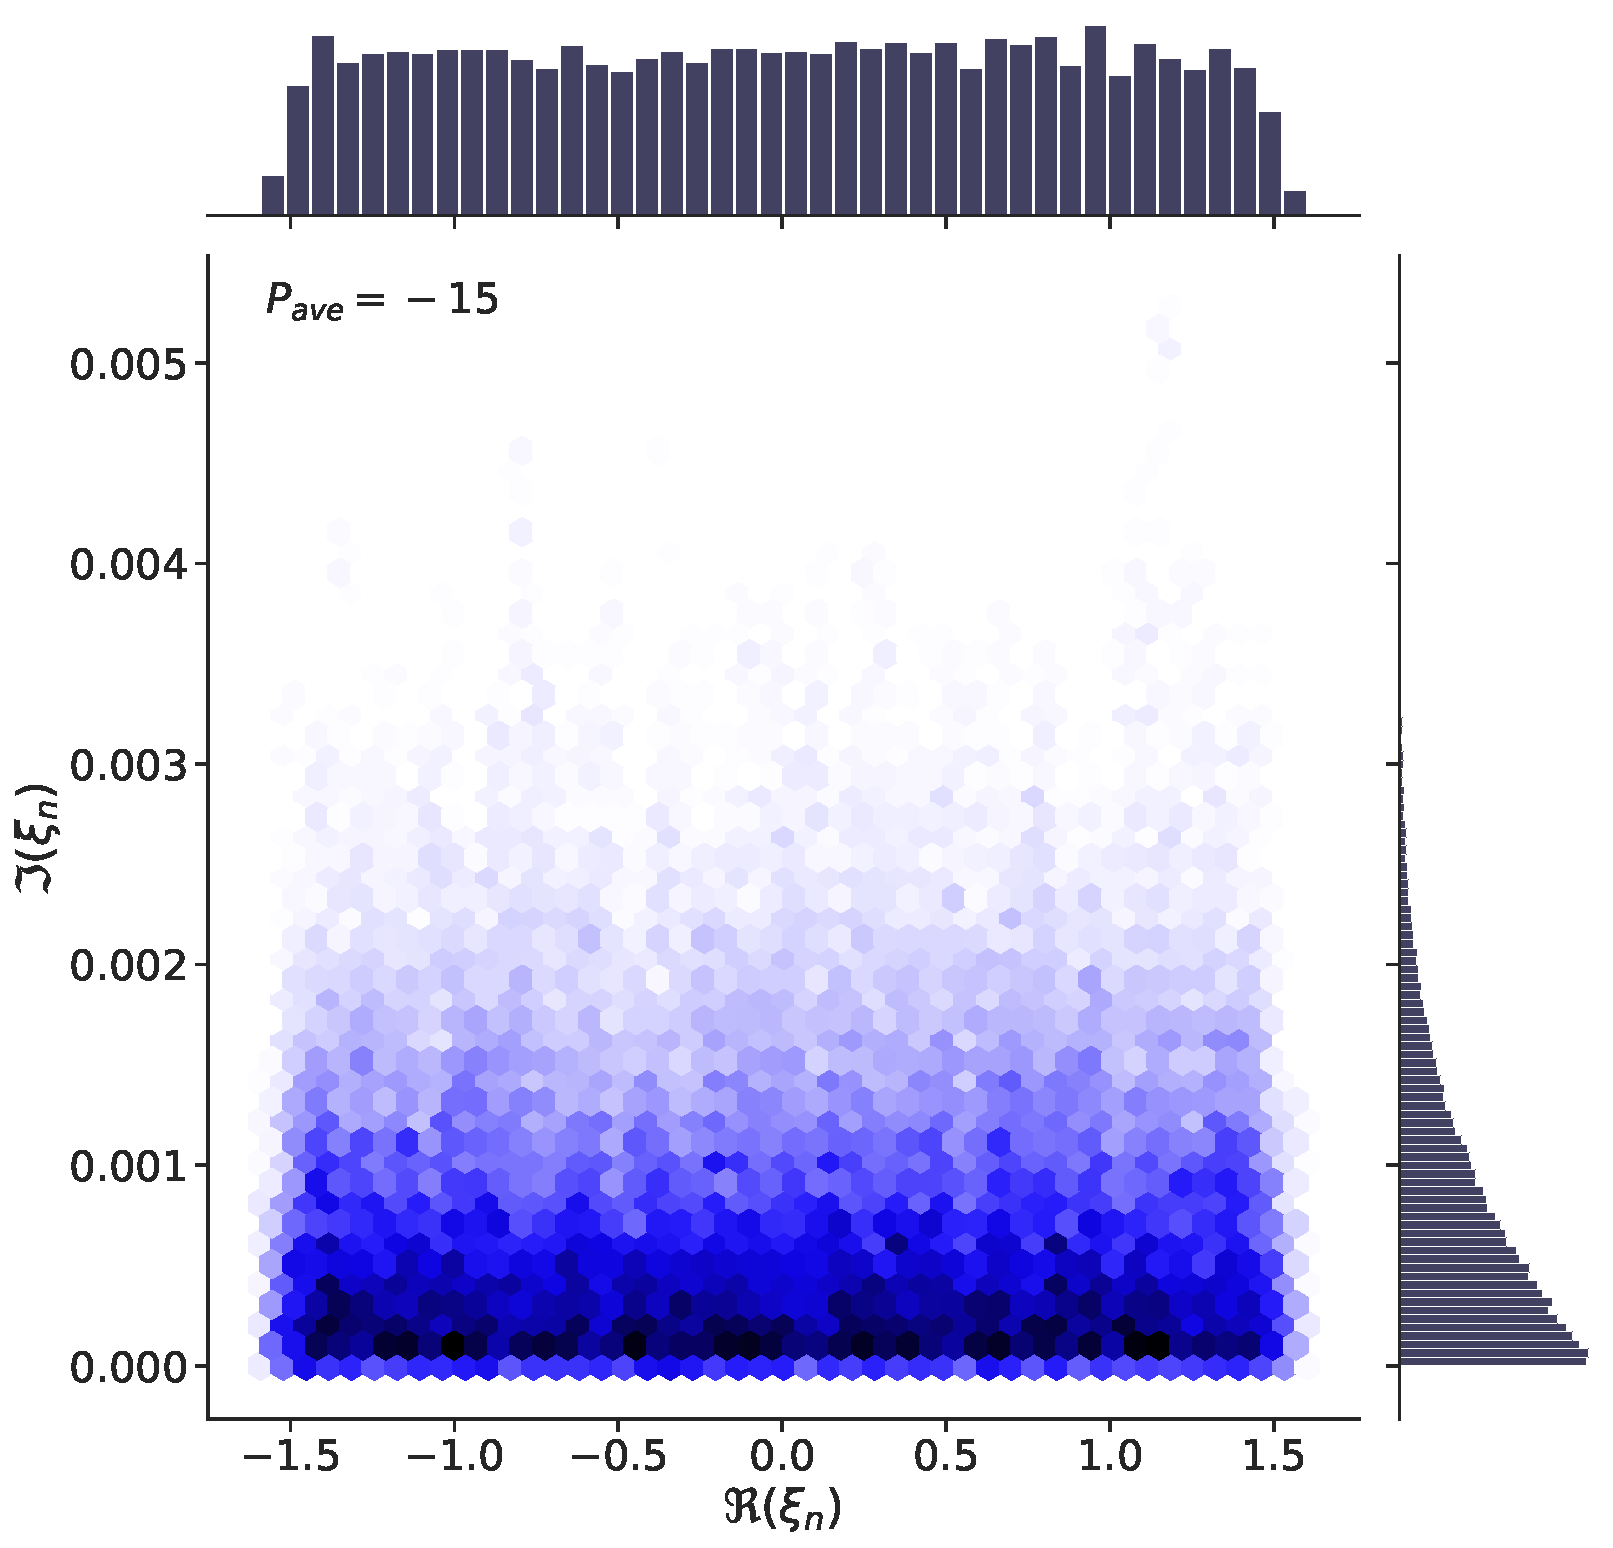
\includegraphics[width=1\linewidth]{images/soliton/wdm_trans/discrete_spectrum_distribution_pavedbm_-15.pdf} \\
    }
    \end{minipage}
    \hfill
    \begin{minipage}[h]{0.49\linewidth}
    \center{
        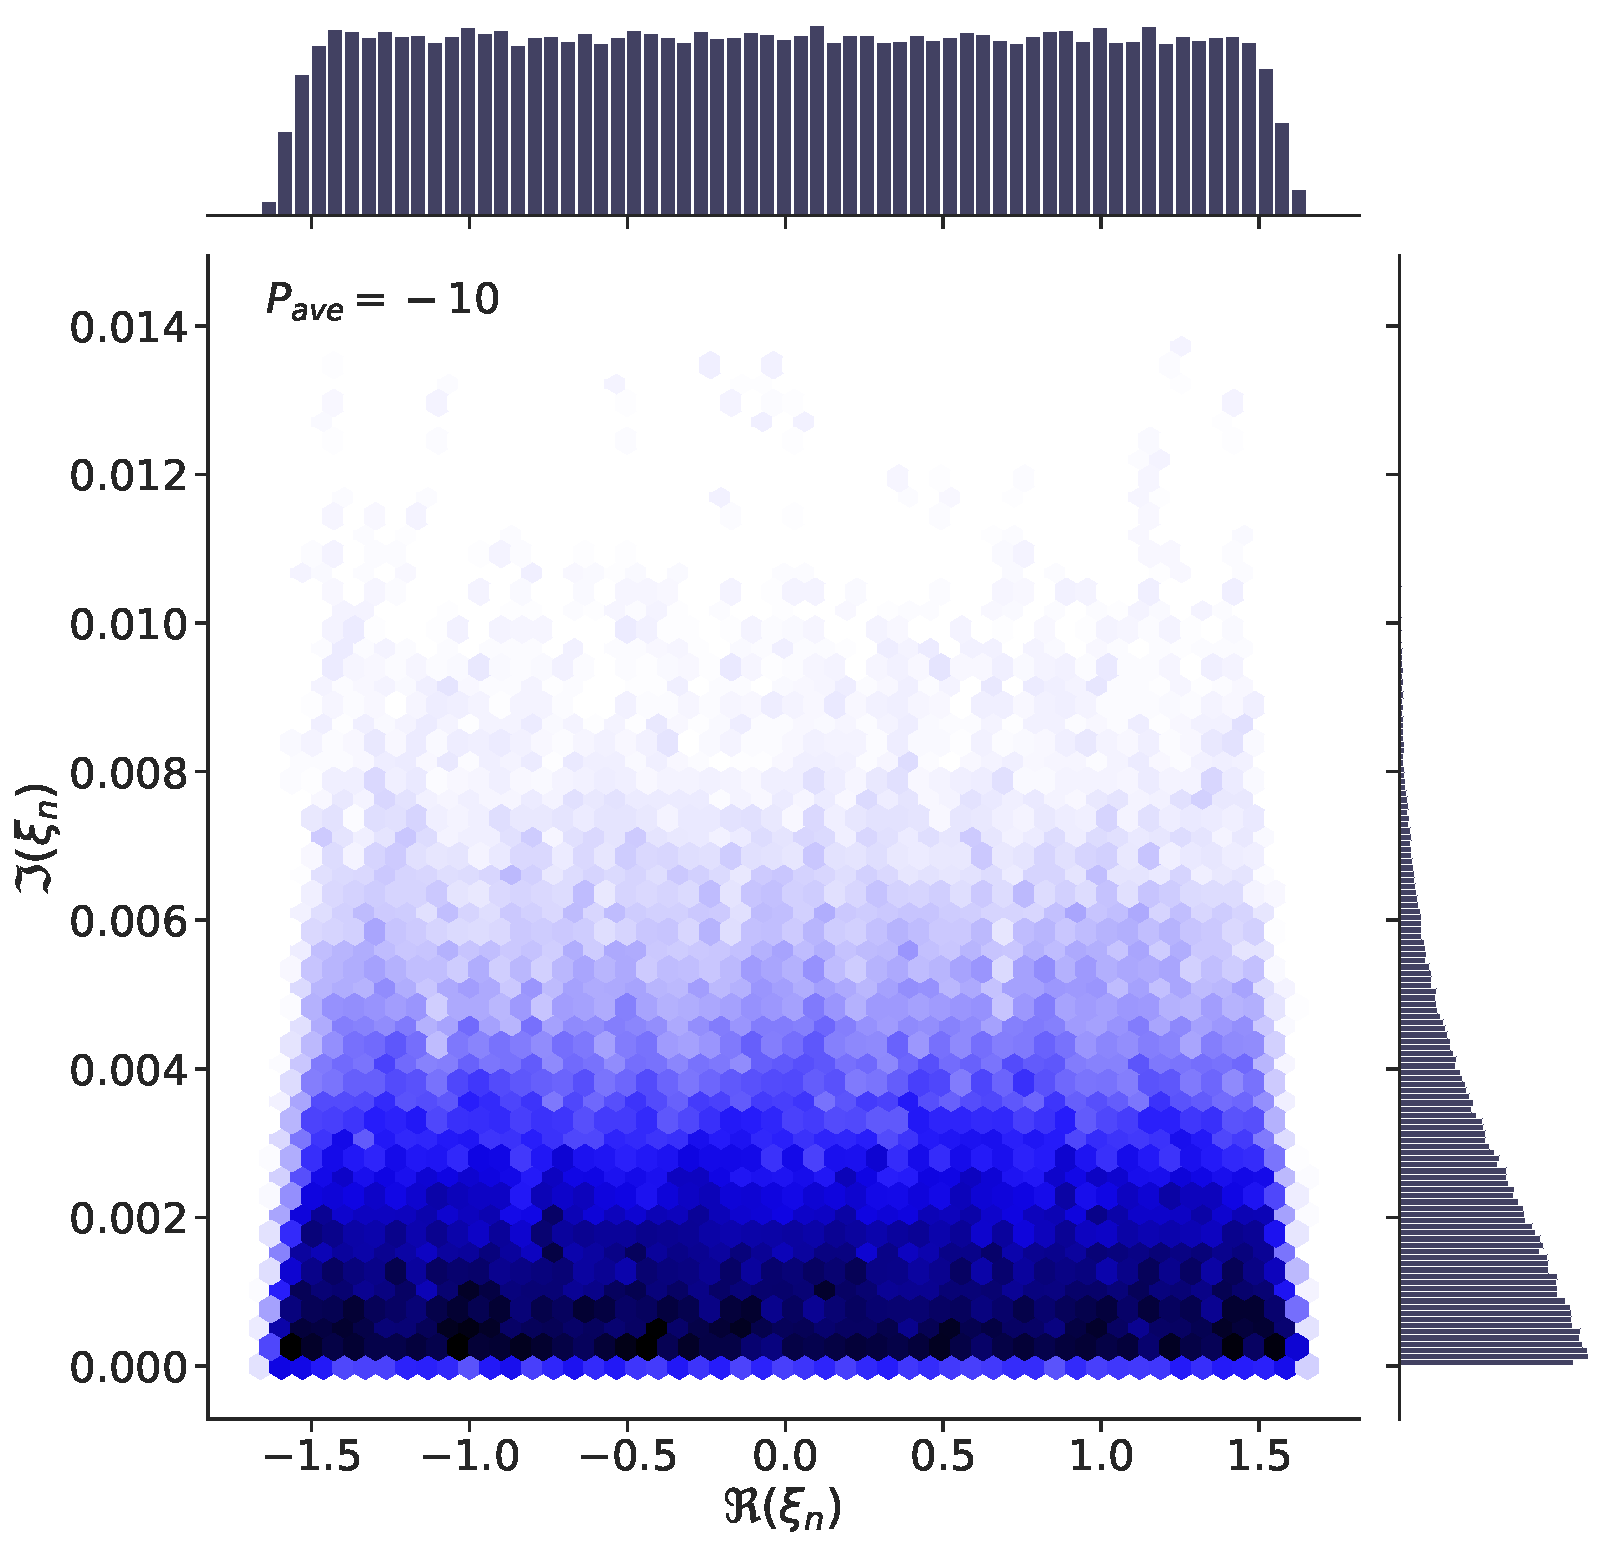
\includegraphics[width=1\linewidth]{images/soliton/wdm_trans/discrete_spectrum_distribution_pavedbm_-10.pdf} \\
    }
    \end{minipage}

    \begin{minipage}[h]{0.49\linewidth}
    \center{
        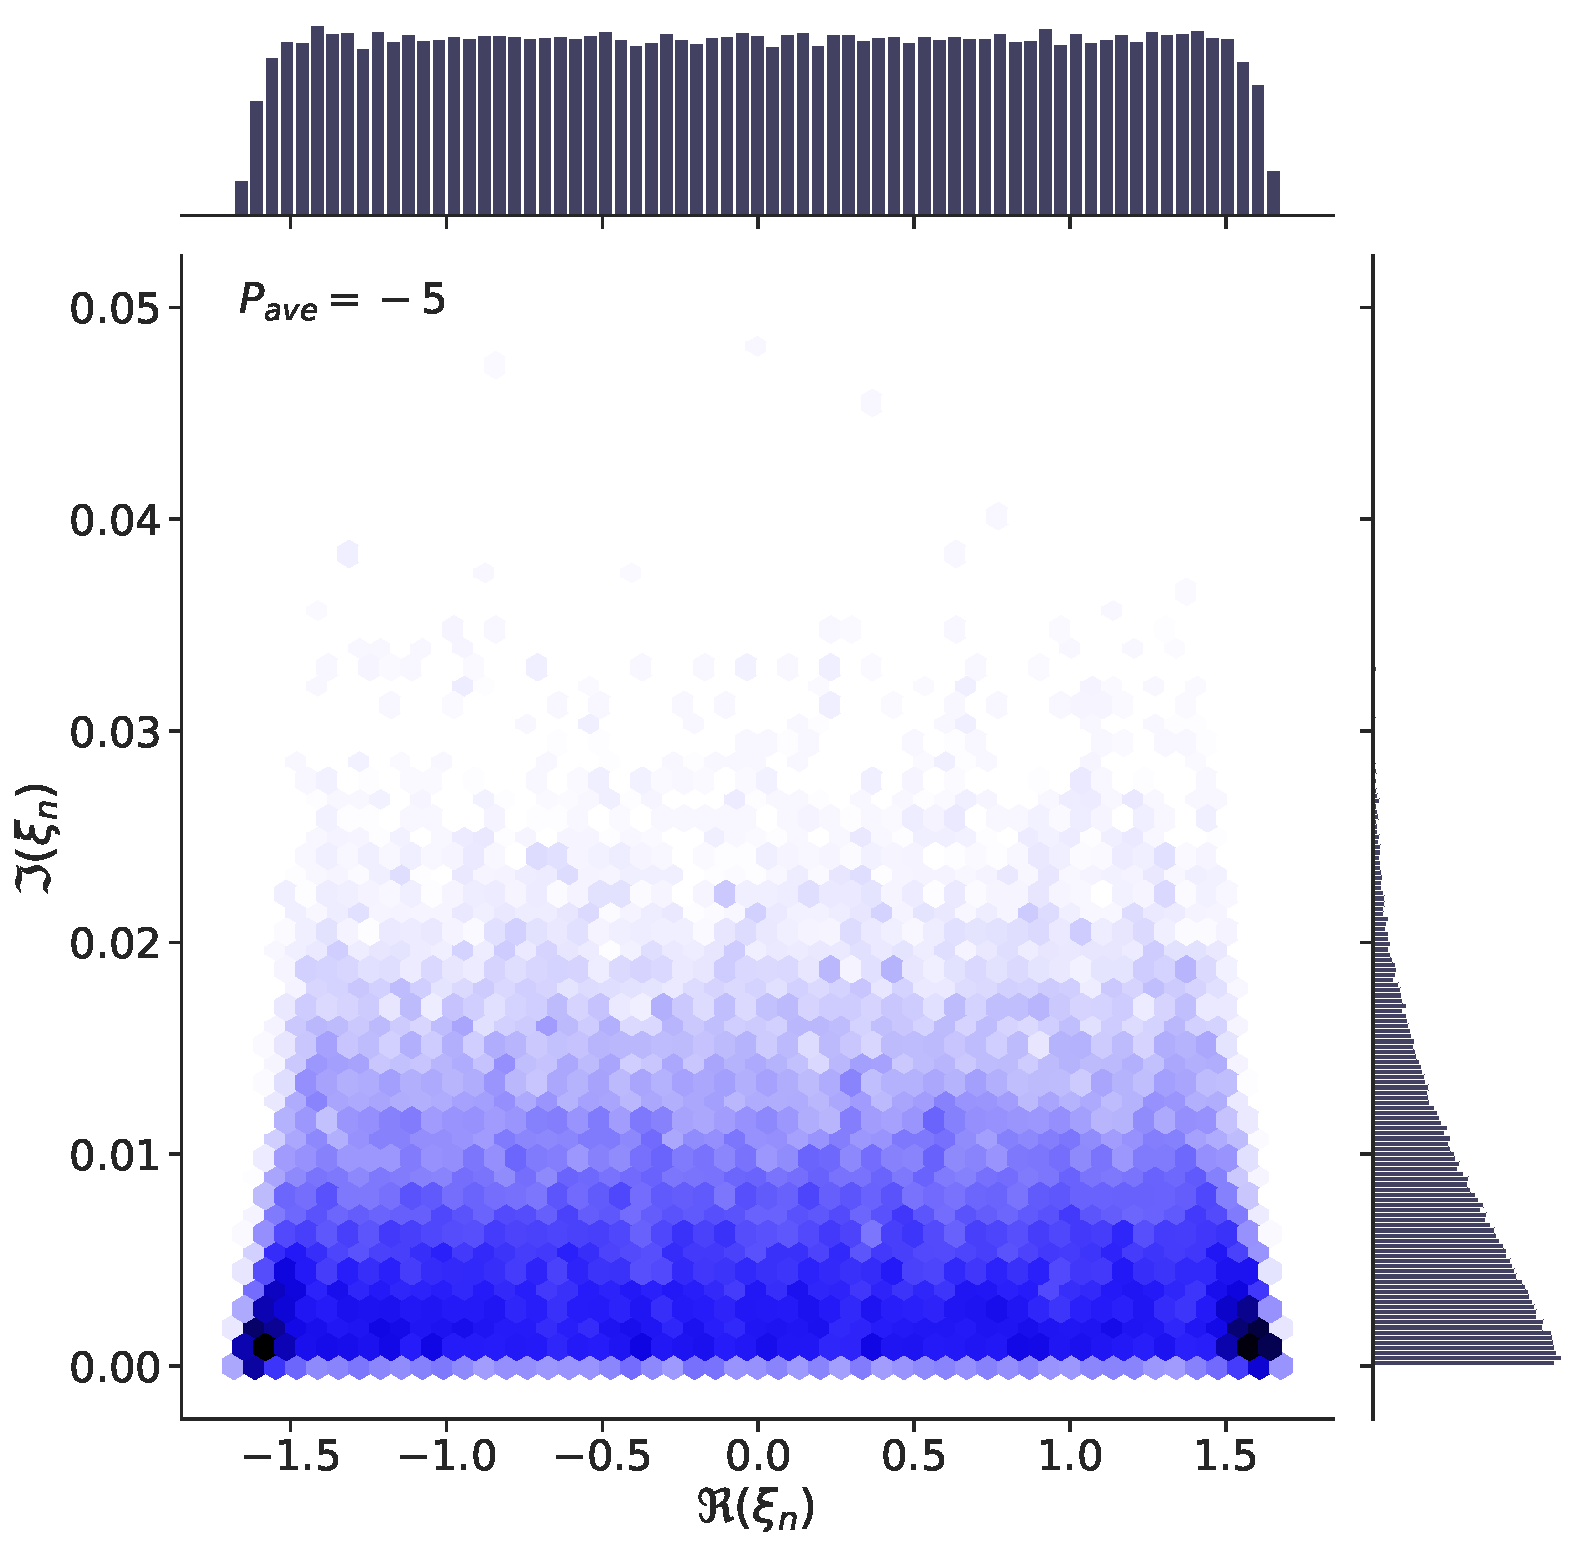
\includegraphics[width=1\linewidth]{images/soliton/wdm_trans/discrete_spectrum_distribution_pavedbm_-5.pdf} \\
    }
    \end{minipage}
    \hfill
    \begin{minipage}[h]{0.49\linewidth}
    \center{
        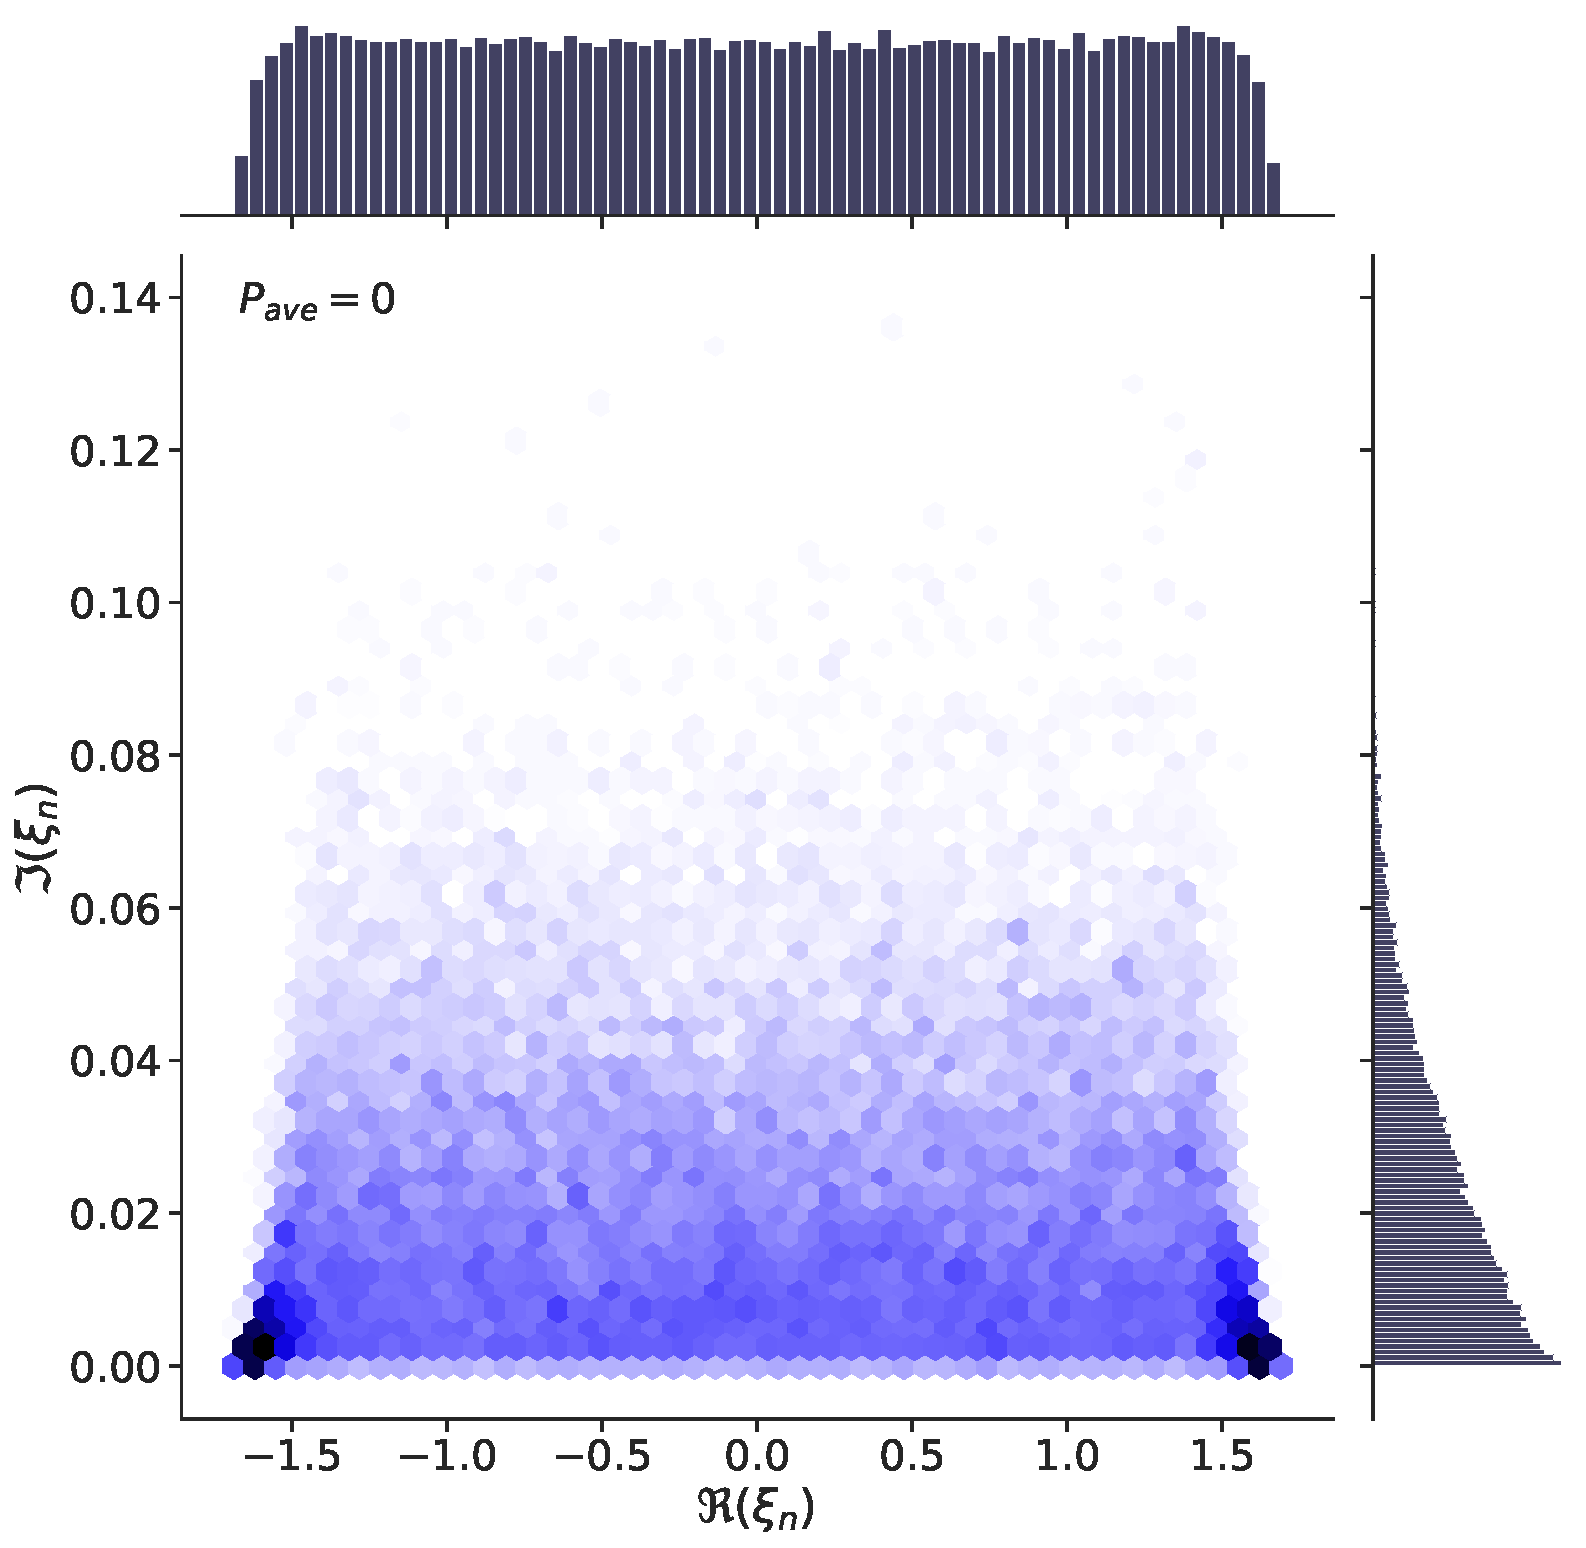
\includegraphics[width=1\linewidth]{images/soliton/wdm_trans/discrete_spectrum_distribution_pavedbm_0.pdf} \\
    }
    \end{minipage}

    \begin{minipage}[h]{0.49\linewidth}
    \center{
        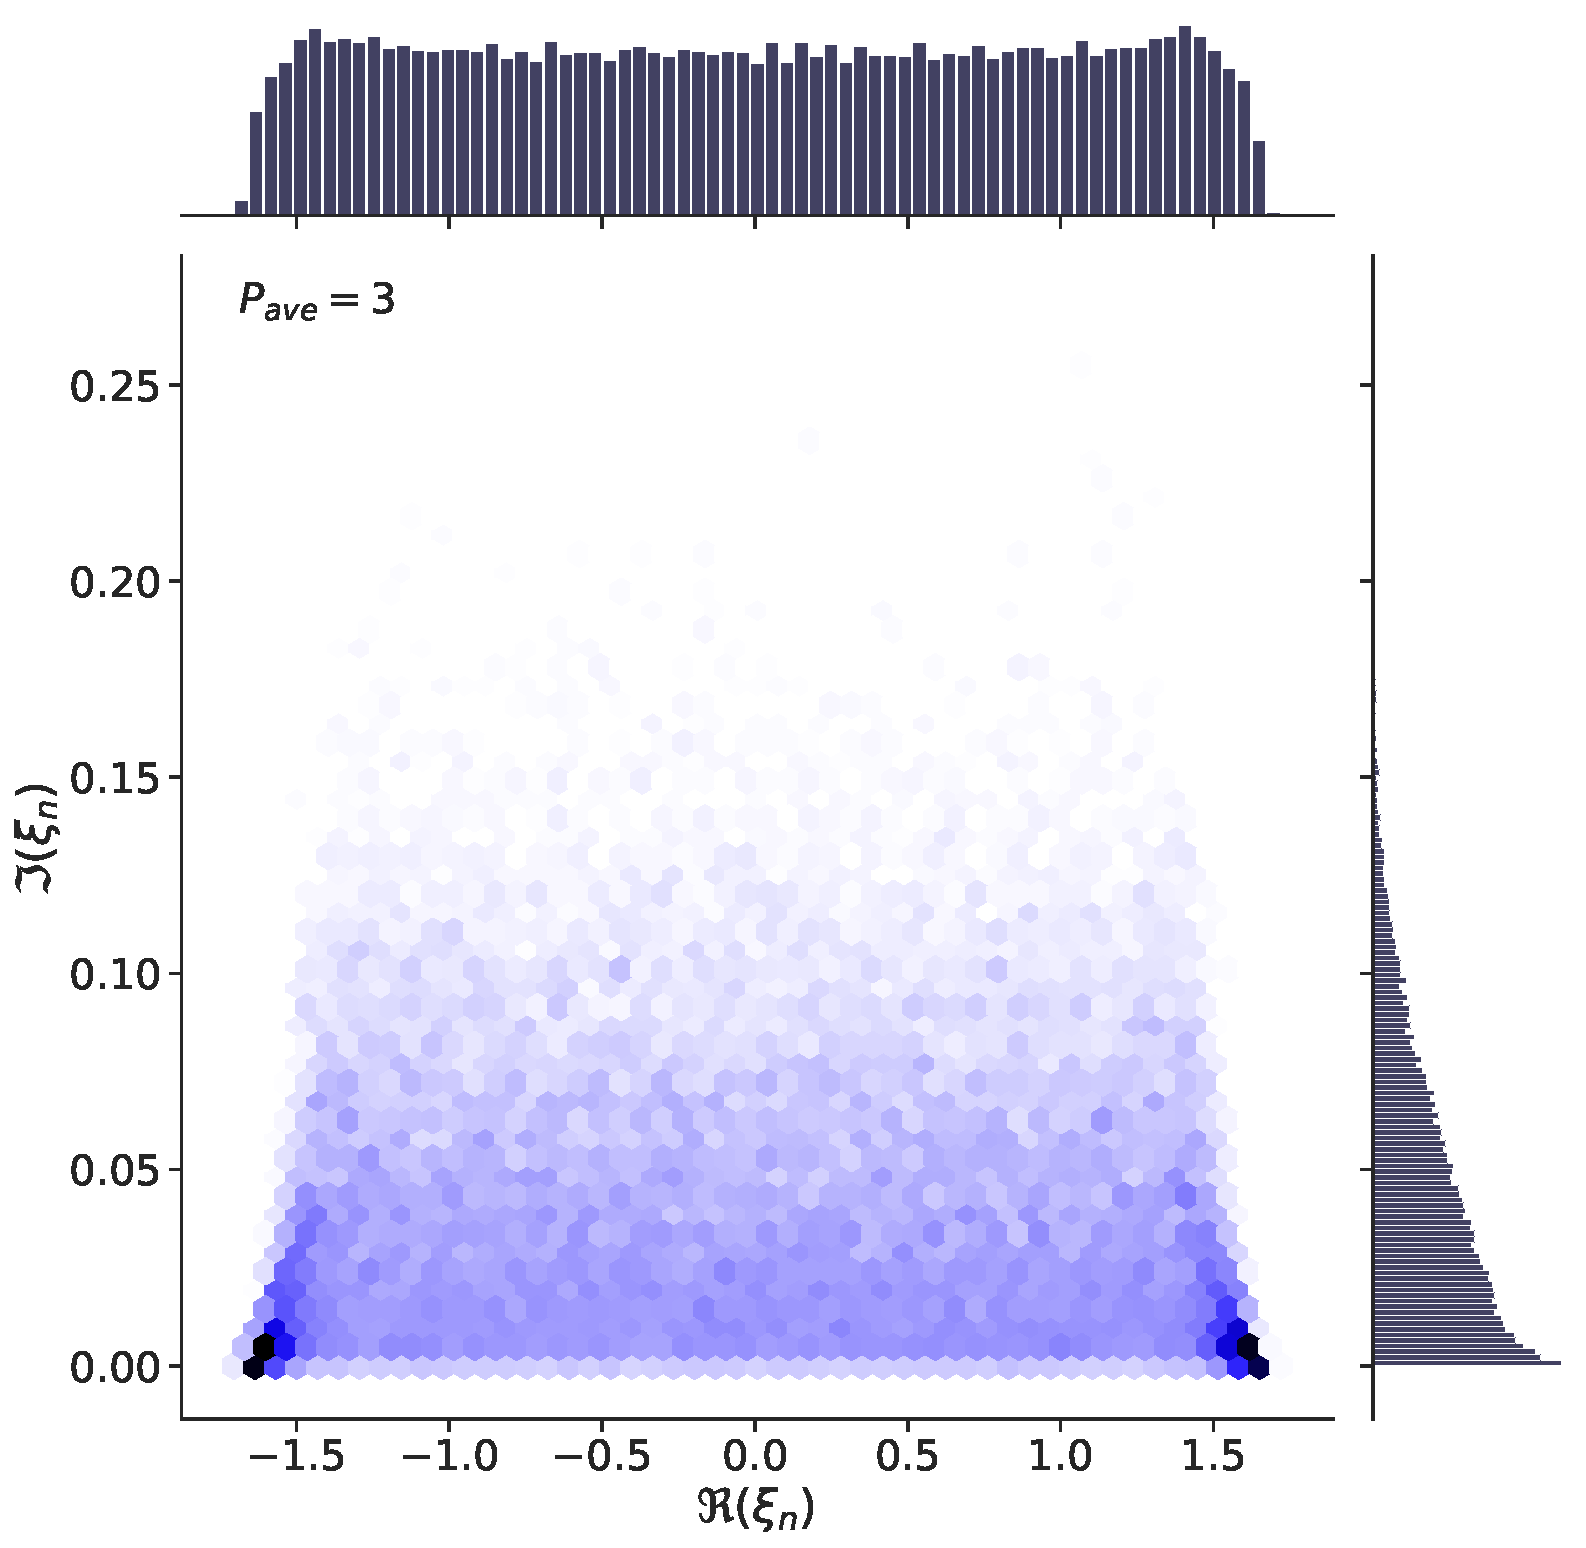
\includegraphics[width=1\linewidth]{images/soliton/wdm_trans/discrete_spectrum_distribution_pavedbm_3.pdf} \\
    }
    \end{minipage}
    \hfill
    \begin{minipage}[h]{0.49\linewidth}
    \center{
        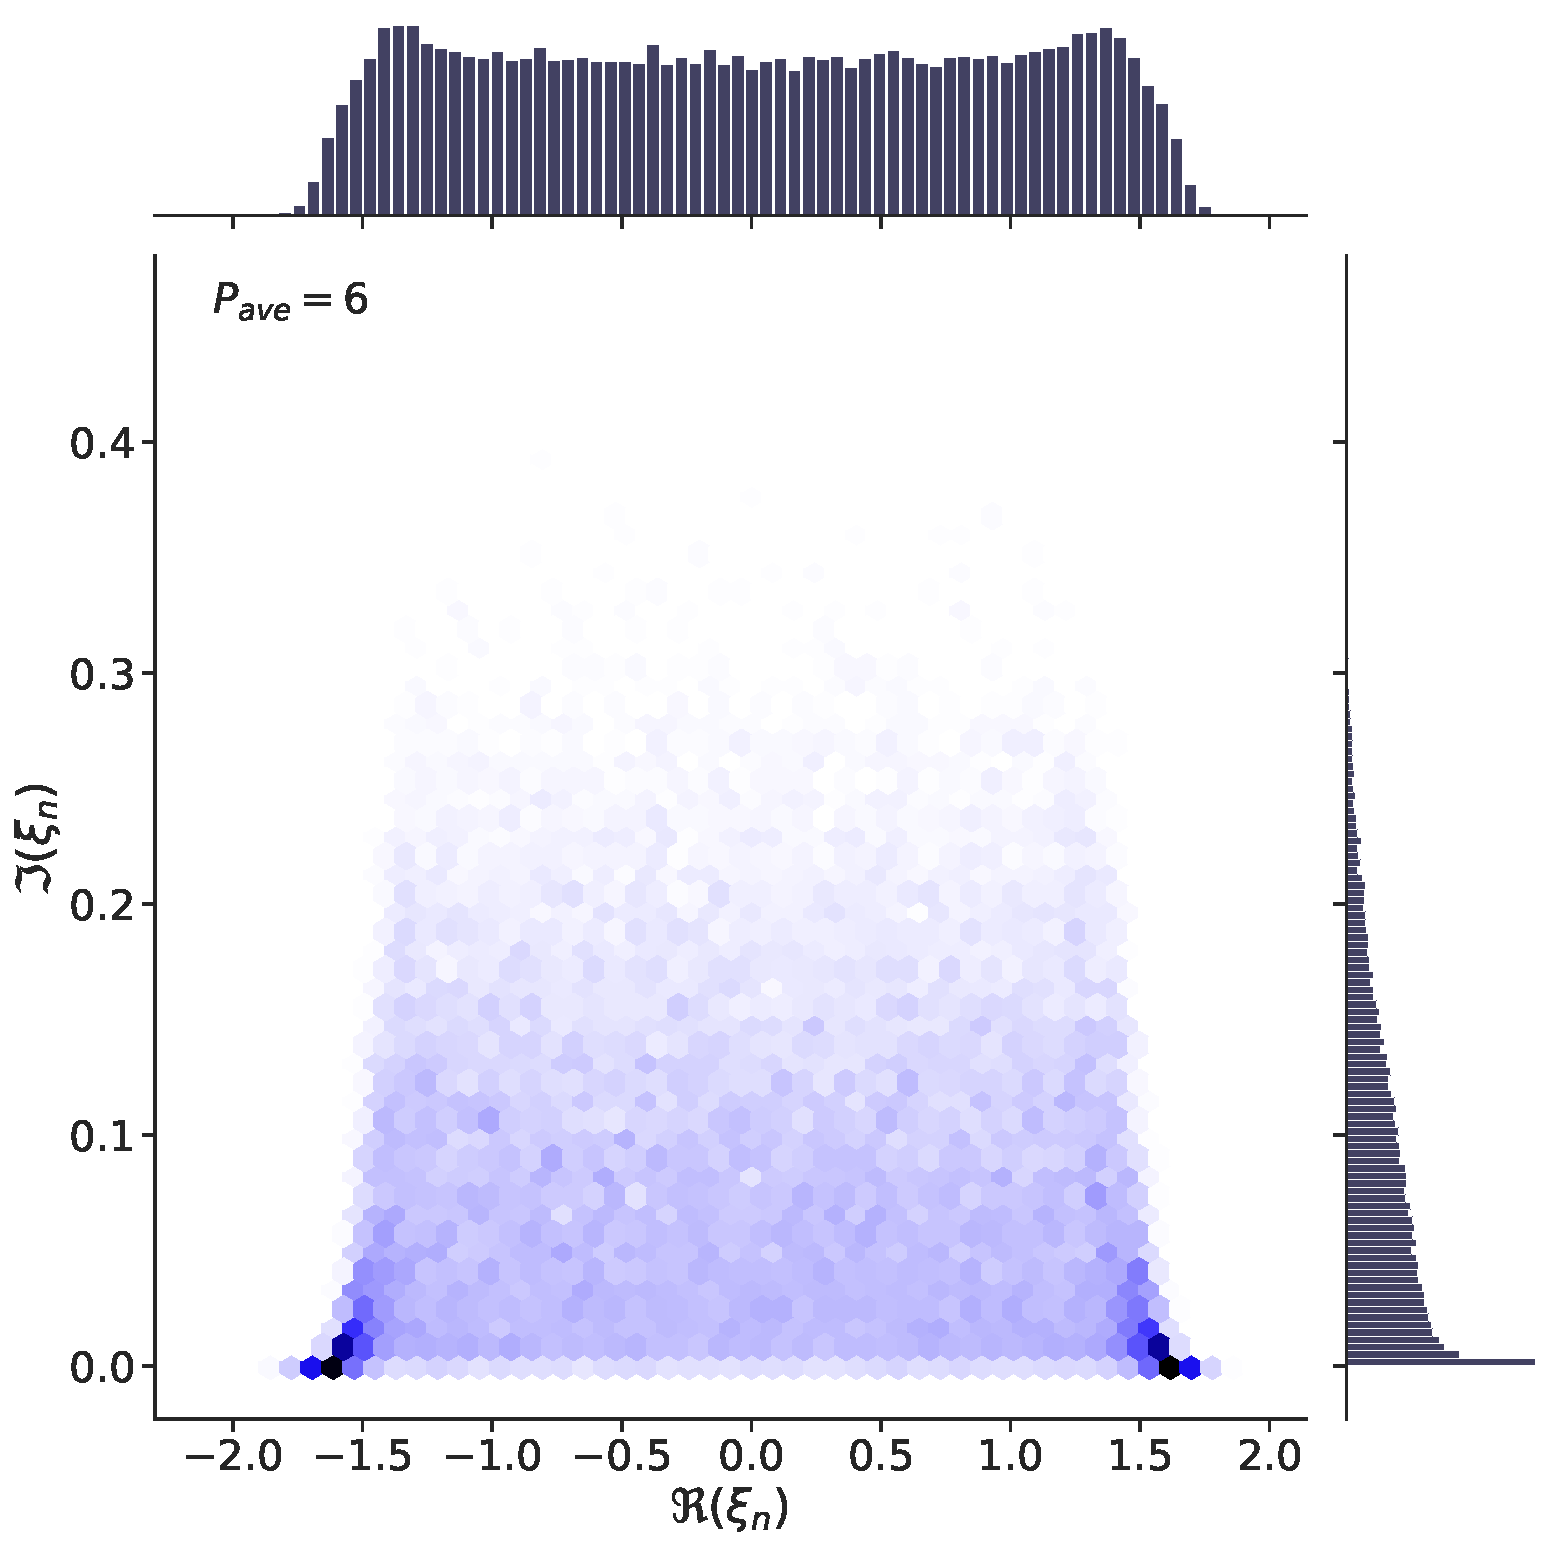
\includegraphics[width=1\linewidth]{images/soliton/wdm_trans/discrete_spectrum_distribution_pavedbm_6.pdf} \\
    }
    \end{minipage}
    \caption{Distribution of discrete eigenvalues in the NF spectrum across the complex plane at varying signal power levels, beginning at -15 dBm in the upper left and concluding at 6 dBm in the lower right panels.}
    \label{fig:wdm_trans_sol_full_distr}
\end{figure}


Figure~\ref{fig:wdm_trans_sol_full_distr} illustrates the distribution of discrete eigenvalues in the NF spectrum across the complex plane at varying signal power levels, beginning at \(-15\) dBm in the upper left and concluding at \(6\) dBm in the lower right panels. The intensity of the blue color represents the density of points within the spectral space. Accompanying the main graph, histograms along the top and right edges display the distributions of the real and imaginary parts, respectively.

At lower power levels, a substantial presence of solitons is evident, with an average count of approximately \(60\) for \(-15\) dBm and about \(214\) for \(-10\) dBm. These figures indicate that the real part of the discrete spectrum is evenly distributed, aside from the spectral edges where the signal's bandwidth limit has an effect. For the imaginary part, the distribution shows a general decline with an increase in the imaginary value, suggesting a higher prevalence of low- and mid-energy solitons over those with high energy. This pattern is consistent even at \(-5\) dBm, as shown in the second row, first panel of Fig.~\ref{fig:wdm_trans_sol_full_distr}.

As the average signal power increases, a notable change occurs: low-energy solitons begin to cluster at the boundaries of the spectral intervals. This clustering is observable at \(0\) dBm and becomes more noticeable at \(3\) and \(6\) dBm, where the right histograms reveal a significant peak near the real axis. Beyond this peak, there is a gradient decrease in the imaginary part of the discrete eigenvalues. In Fig.~\ref{fig:ds_vs_power}, we observed that for average signal powers exceeding \(1\) dBm, the signal reaches a saturation point, with nearly all (\(99\%\)) of its power comprised of solitons. Yet, as the power continues to increase, so does the number of solitons, suggesting an accumulation of lower-energy solitons and a concentration at the spectral interval edges.

The underlying reasons for this tendency are not immediately clear, but from a physical standpoint, it could be assumed that this pattern represents an energy-efficient arrangement of discrete eigenvalues within the spectral space.

